\chapter{Eletrônica}

O subsistema de eletrônica é divido em 3 partes. A primeira parte é composta pelo radar, a segunda pelo sistema de controle embarcado no totem e por fim o processamento de imagens. 
%Colocar diagrama geral totem eletrônica


\section{Sistema do radar}
O sistema do radar é responsável por realizar a transmissão e recepção do sinal através do qual é possível detectar objetos e calcular sua velocidade com relação ao radar.

O tipo de radar utilizado foi um \textit{Continuous-Wave Radar (CW Radar)}, como mostra a Figura \ref{Doppler1}, sendo este caracterizado por uma emissão contínua do sinal em alta frequência pela antena, onde a mesma deve ser direcionada para o alvo com intuito do sinal ser transmitido e recebido na mesma região. 

O radar CW é caracterizado por não apresentar nenhum tipo de modulação, com isso é possível mensurar somente a velocidade de alvos que se aproximem ou se afastem do radar. O cálculo da velocidade é realizada através do efeito  \emph{Doppler}, fenômeno físico no qual a frequência central do sinal é deslocada no espectro quando o mesmo é refletido por um objeto que possui uma velocidade com relação ao radar. 
\begin{figure}[H]
    \centering
   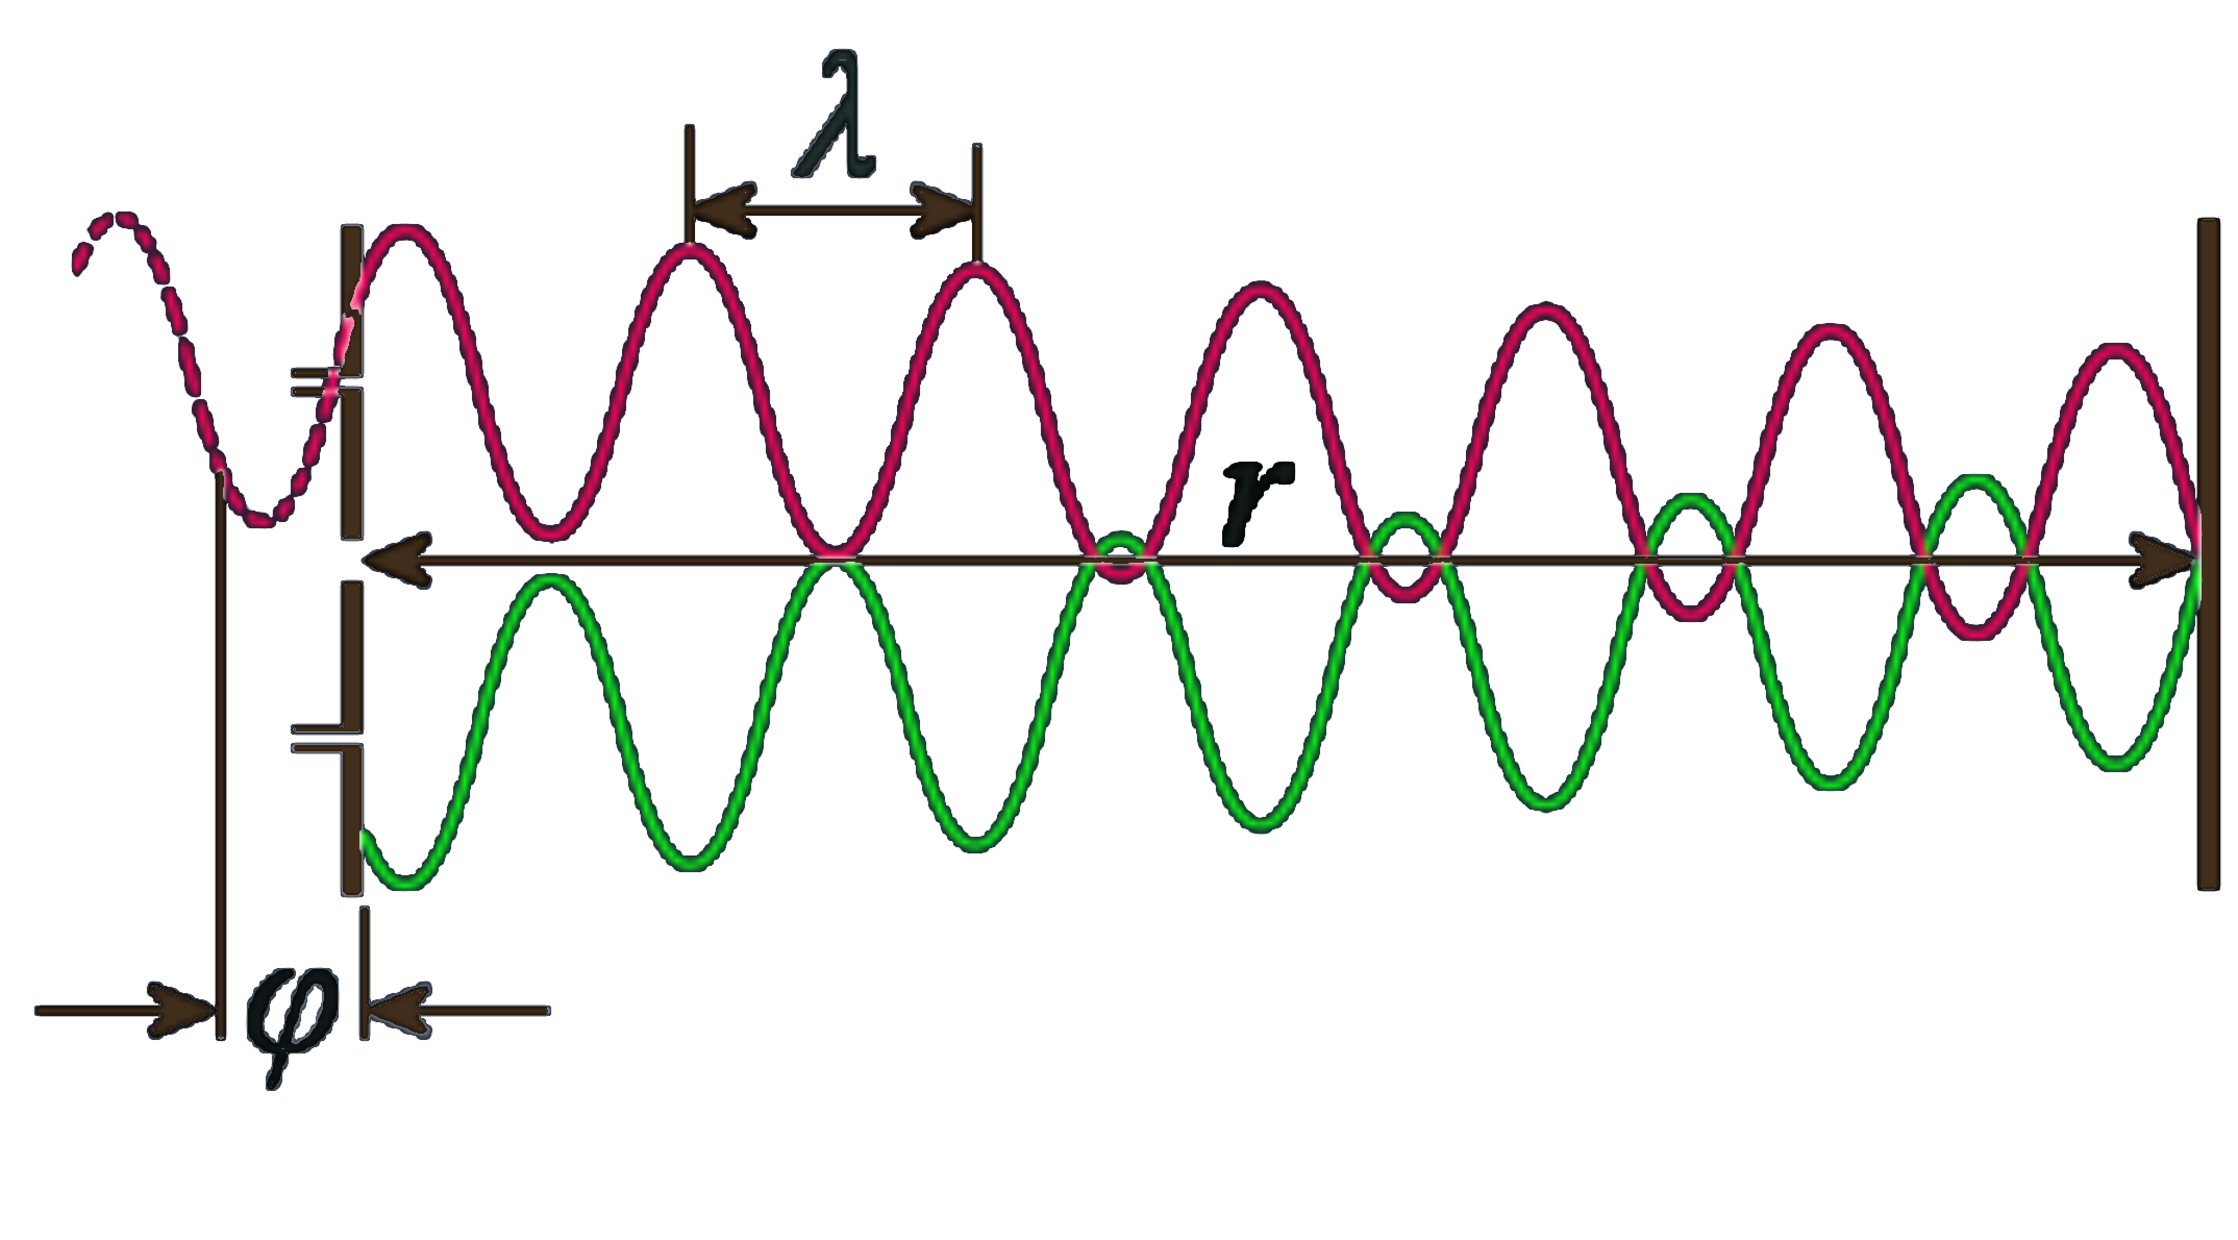
\includegraphics[scale = 0.25]{figuras/Doppler2.pdf}
   \caption{Diferença de fase entre o sinal transmitido e recebido.}
   \label{Doppler1}
    \end{figure}

O radar de onda contínua avalia a relação entre a fase $\phi$ da onda transmitida e recebida. A relação entre a magnitude do sinal na recepção pode ser calculada de acordo com a distância percorrida pela onda eletromagnética e também pelo comprimento de onda do sinal transmitido. Considerando uma distância constante de um alvo até radar, podemos descrever a seguinte relação: 

\begin{equation}
    \label{fase_1_doppler}
    \phi = -2\pi\frac{2r}{\lambda},
\end{equation}
Onde:
\begin{itemize}
    \item $\phi$= Diferença de fase entre os sinais transmitido e recebido;
    \item $r$= Distância percorrida pela onda;
    \item $\lambda$= Comprimento de onda do sinal transmitido;
\end{itemize}

O fator $2r$ dentro da equação se deve ao fato das ondas eletromagnéticas terem que percorrer a distância até o alvo, serem refletidas pelo mesmo para serem captadas pela antena posicionada no radar \cite{Doppler}. Pelo fato de não haver sido modulado o sinal a distância entre o alvo e o radar não pode ser calculada devido a ambiguidade ocasionada pelo comprimento de onda, onde o mesmo varia entre $0$ e $2\pi$. Se a distância do alvo até o radar não for constante, podemos representar a relação expressa na Eq.\ref{fase_1_doppler} da seguinte forma:

\begin{equation}
    \label{fase_2_doppler}
    \phi(t) = -4\pi\frac{r(t)}{\lambda}.
\end{equation}

Sabendo que o alvo está variando a sua posição com relação ao radar ao longo do tempo, basta derivar a Eq.\ref{fase_2_doppler}, que com isso podemos encontrar a velocidade relativa do alvo com relação ao radar:

\begin{equation}
    \label{fase_3_doppler}
    \frac{d\phi(t)}{dt} = -4\pi\frac{dr(t)}{dt\lambda},
\end{equation}

\begin{equation}
    \label{fase_4_doppler}
    \omega(t) = -4\pi\frac{v(t)}{\lambda},
\end{equation}

\begin{equation}
    \label{fase_5_doppler}
    v(t) = \frac{\omega(t)\lambda}{-4\pi}.
\end{equation}

De acordo com a Eq. \ref{fase_5_doppler} podemos verificar a relação entre a velocidade de objetos que se movimentam na região de campo captada pela antena e a velocidade angular da onda eletromagnética na recepção do radar, porém a velocidade do alvo relacionado a variação de fase da onda na recepção é conhecida como velocidade radial, velocidade radial é a velocidade do alvo que se movimenta de acordo com o campo de visada podendo ser definida também como a velocidade com a qual o objeto se aproxima de um determinado observador, sendo ela calculada como:

\begin{equation}
    \label{V_r}
    v_r(t) = v(t)cos\theta,
\end{equation}

\begin{equation}
    \label{V_r}
    v(t) = \frac{v_r(t)}{cos\theta}.
\end{equation}

Onde:
\begin{itemize}
    \item $V_r(t)$: Velocidade radial do alvo com relação ao radar;
    \item $V(t)$: Velocidade do alvo;
    \item $\theta$: Ângulo entre o vetor velocidade e a distância até o radar.
\end{itemize}


\subsection{Antena}

As antenas utilizadas no projeto são antenas dipolo de polarização linear, frequência central de 915 MHz e com uma largura de banda de 26 MHz, onde as duas antenas são idênticas, portanto, todas as propriedades são iguais. A Figura \ref{antena} mostra uma das antenas que foram utilizadas. 

\begin{figure}[H]
    \centering
   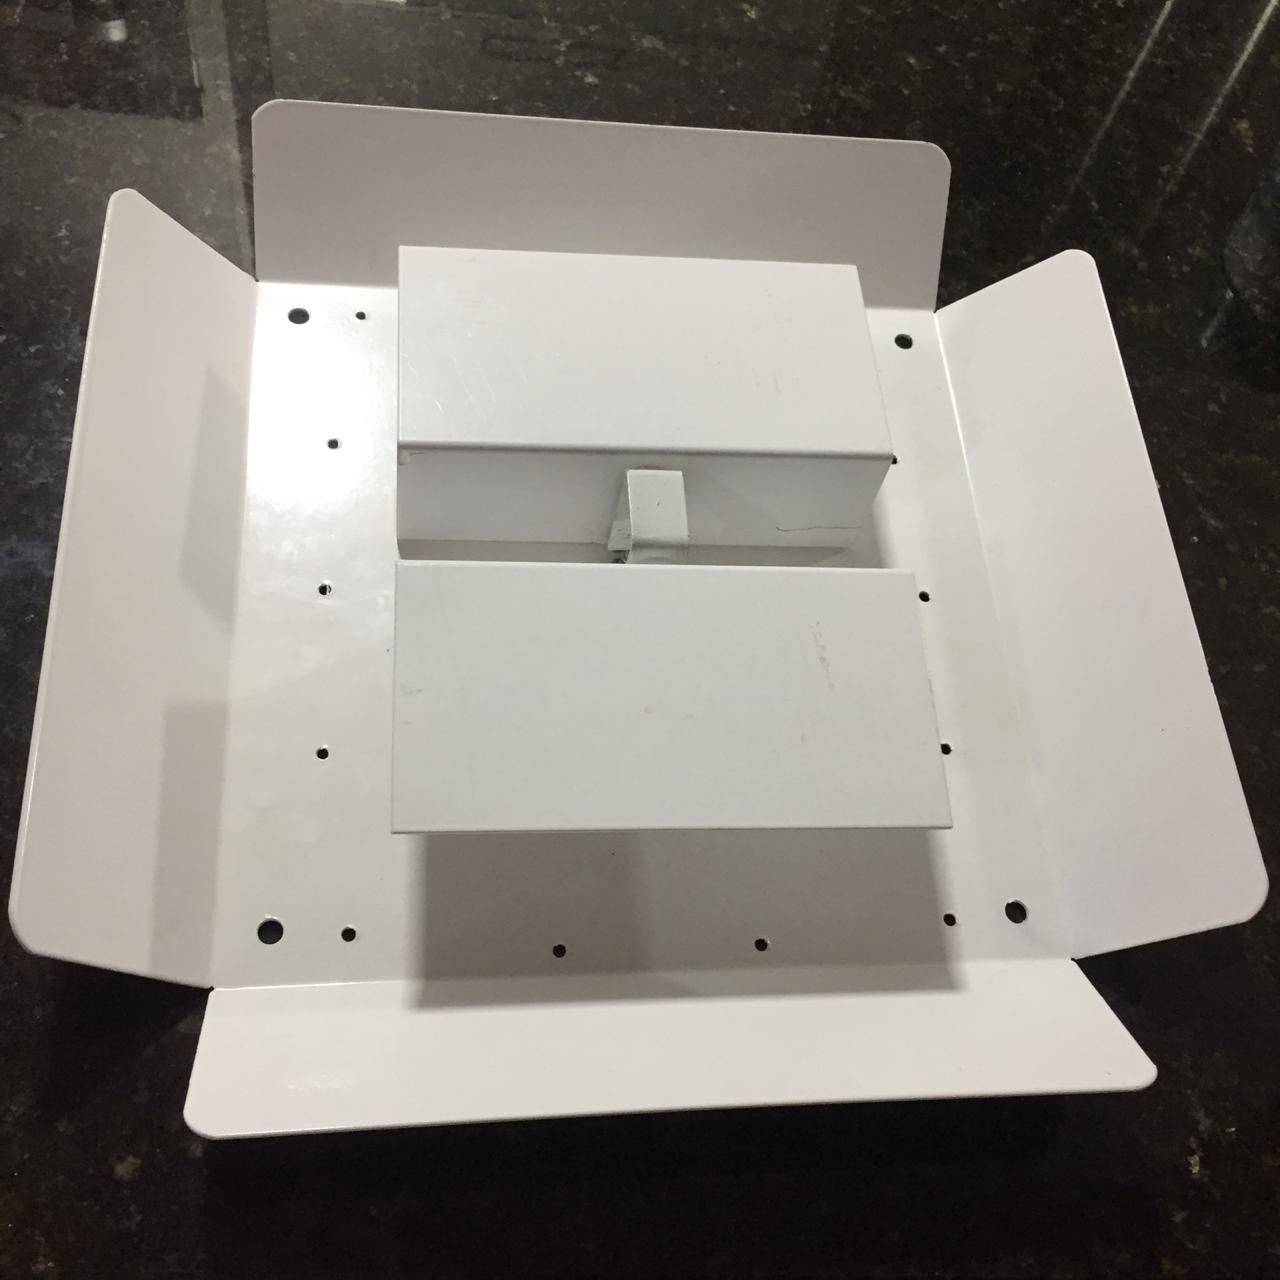
\includegraphics[scale = 0.15]{figuras/antena.jpeg}
   \caption{Antena dipolo com frequência central de 915MHz que é utilizada para a transmissão e recepção de dados no radar.}
   \label{antena}
    \end{figure}

Outros parâmetros importantes das antenas são sua diretividade, ou seja, a capacidade de focalizar energia em um ponto, e também o ganho da antena. Neste caso a antena possuiu um ganho e diretividade de 9 dB, como mostrado na Figura \ref{ganho}. 

\begin{figure}[H]
    \centering
   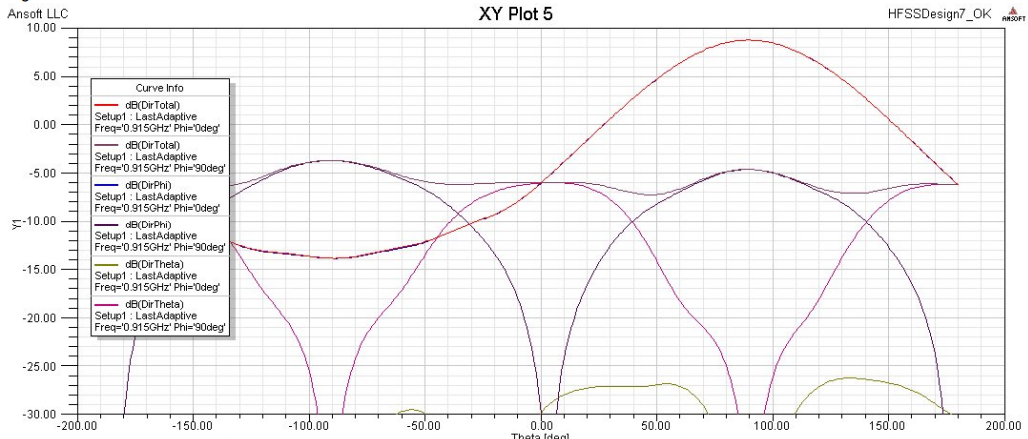
\includegraphics[scale = 0.45]{figuras/ganho.png}
   \caption{Diagrama de radiação com o ganho da antena.}
   \label{ganho}
    \end{figure}

Podemos verificar também a abertura de 3 dB das antenas, onde está concentrado metade da energia transmitida ou recebida pela antena. Para calcular este ângulo é preciso pegar o maior valor no diagrama de radiação e deslocar 3 dB no eixo das ordenadas, sendo a abertura 3 dB a variação angular contida nessa região. Esse dado pode ser verificado tanto no diagrama disponibilizado pelo fabricante, na Figura \ref{ganho}, onde se encontra na faixa dos 50$^{\circ}$ a 120$^{\circ}$ como no diagrama caracterizado em campo onde a mesma abertura se encontra na faixa de -35$^{\circ}$ a 35$^{\circ}$, como na Figura \ref{dr}, confirmando que a antena utilizada possui uma abertura 3 dB de 70$^{\circ}$. 

\begin{figure}[H]
    \centering
   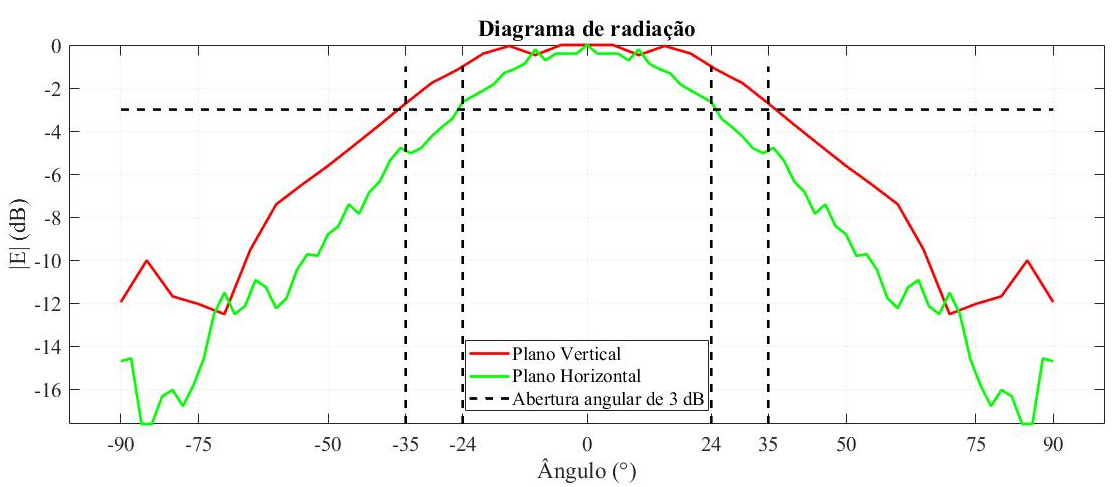
\includegraphics[scale = 0.3]{figuras/gir.png}
   \caption{Diagrama de radiação da antena e a
abertura 3 dB, caracterizada na faculdade.}
   \label{dr}
    \end{figure}


\subsection{Parâmetros do radar}


 Por se tratar de um radar que tem como objetivo mensurar a variação de frequência através do efeito \emph{Doppler}, um dos parâmetros necessários para se estabelecer o correto funcionamento do sistema é o cálculo da variação em frequência que se dá através da Eq. \ref{Doppler0} de efeito \emph{Doppler}\cite{young2009fisica}.
%Nussenzveig, Moysés, H. Curso de Física Básica. [Minha Biblioteca]. Retirado de https://integrada.minhabiblioteca.com.br/#/books/9788521208044/
\begin{equation}\label{Doppler0} 
  f_0 = f_f \Big(\frac{c \pm v_0}{c \mp v_f} \Big)
\end{equation} 

Onde $f_0$ é a frequência observada pelo observador, $f_f$ é a frequência emitida pela fonte, \emph{c} é a velocidade da luz, $v_0$ é a velocidade do observador em relação ao meio, sendo esta positiva ao se aproximar da fonte e negativa ao se afastar, $v_f$ é a velocidade da fonte em relação ao meio, sendo positiva ao se afastar e negativa ao se aproximar do observador.

Como a velocidade do observador representa a velocidade do radar e o mesmo se encontra fixo na rodovia, então $v_0$ é considerado como sendo 0, resultando na Eq. \ref{Doppler0-1}.
%Nussenzveig, Moysés, H. Curso de Física Básica. [Minha Biblioteca]. Retirado de https://integrada.minhabiblioteca.com.br/#/books/9788521208044/
\begin{equation}\label{Doppler0-1} 
  f_0 = f_f \Big(1 + \frac{v_f}{c} \Big)
\end{equation}

A partir da relação $\Delta f = f_{f} - f_{0}$, podemos concluir que a variação de frequência é dada através da Eq. \ref{Doppler}.

\begin{equation}\label{Doppler} 
  \Delta f =  \frac{2v_f}{\lambda}
\end{equation} 

Onde $\Delta f$ representa a variação de frequência do sinal, $v_f$ representa a velocidade relativa do alvo com relação ao radar e $\lambda$ é o comprimento de onda do sinal emitido pela antena. Como $\lambda$ depende exclusivamente da frequência do sinal emitido e o mesmo se encontra na faixa dos 915 MHz, utilizando a relação $f=c/\lambda$  podemos encontrar um valor para $\lambda$ de 0.328m. Substituindo na Eq. \ref{Doppler}, temos que $\Delta f = 6.1 Hz$.

De acordo com este resultado, uma variação de $1 m/s$ na velocidade da fonte para o radar é representada por um desvio de $6.1 Hz$. Utilizando uma variação em $km/h$ para representar a velocidade da fonte dividimos o resultado anterior por um fator de 3.6 de modo que uma variação de $1km/h$ pode ser visualizada através de um desvio de $1.7 Hz$.

Um outro fator importante para se estabelecer a variação em frequência é o ângulo entre a direção de transmissão/recepção do sinal e a trajetória do alvo, de modo que a equação \ref{Doppler} é alterada de acordo com o ângulo $\theta$ mensurado, mostrada na Eq. \ref{Doppler2} \cite{radarbasics}.
%http://www.radartutorial.eu/11.coherent/co06.en.html

 \begin{equation}\label{Doppler2} 
  \Delta f =  \frac{2v}{\lambda}cos \theta
\end{equation}

Isso implica que a variação estabelecida na Eq \ref{Doppler} é dada como sendo a máxima para um alvo que se aproxima do radar. Quando o objeto se encontra muito distante do radar esse ângulo se torna muito pequeno e a variação causado por ele inexpressiva, porém de acordo com que o alvo se aproxima, pode ser um fator determinante no cálculo da velocidade do alvo.

Outro parâmetro é a distância máxima que o radar vai conseguir detectar um veículo, pois é necessário alertar ao motorista que vem em direção oposta a possibilidade de uma colisão frontal. Sendo necessária a capturar da imagem do automóvel caso o mesmo ultrapasse a velocidade limite da via. De acordo com esses parâmetros foi definido uma distância de 100 m atendendo o tempo necessário para realizar os processos embarcados no totem, entre eles o cálculo da velocidade do veículo e o comando para captura da imagem. Uma vez estipulada a distância máxima para captura foi possível realizar o cálculo dos demais parâmetros.

%%%%%%%%%parametrôs de potencia e ruido%%%%%%%%%%%%%%
A Eq. \ref{potencia_recebida} define a potência a ser recebida em função do ganho da antena, distância do alvo, da potência transmitida, do comprimento da onda transmitida e da área de seção transversal do alvo \cite{richards2010principles}.

\begin{equation}\label{potencia_recebida}
    P_t\, =\,   P_r \frac{(4\pi)^{3}\,  R^{}4}{G^{2}\,   \lambda^{2}\, \sigma }
\end{equation}%

Onde $P_t$ é a potência transmitida, $P_r$ a potência recebida, $G$ o ganho da antena, $\lambda$ o comprimento de onda do sinal a ser enviado, $\sigma$ a área de seção transversal média do alvo e $R$ a distância do alvo até a antena.

Através das informações acerca da USRP-NI2901 \cite{rds} a potência miníma no canal de recepção RX é de -85 dBm, porém para realização dos cálculos foi estipulado uma sinal na recepção com potência de -50 dBm utilizando os dados onde: $R=100 \, m$, $G=9 \, dB$ Fig.\ref{antena}, $\lambda=0.328 \, m$, a Eq. \ref{Doppler} e $\sigma=1 \, m^{2}$ \cite{richards2010principles}. A partir desses dados e da Eq. \ref{potencia_recebida} podemos chegar a um resultado de $P_t=14.66 \, dBm$ de potência necessária para enviar o sinal a um alvo localizado a 100 m.

A potência de ruído térmico, predominante no projeto é definida na Eq. \ref{potencia_ruido}, onde $P_n$ é a potência de ruído, definida no receptor, $k$ a constante de Boltzman = $1.38 \times 10^{-23} \, J/K$ , $T_e$ a temperatura equivalente de ruído e $B$ a largura de banda \cite{richards2010principles}.

\begin{equation}\label{potencia_ruido}
    P_n = k\, T_e\,B
\end{equation}

A temperatura equivalente de ruído, $T_e$, corresponde a soma da temperatura equivalente de ruído da antena, aqui estimada como temperatura ambiente, 290 K, com a temperatura equivalente de ruído do sistema eletrônico, aqui considerados a relação entre figura de ruído e temperatura equivalente de ruído para obter, no final, uma temperatura equivalente de ruído do sistema de 1453 K. De acordo com esses dados encontrou-se uma potência de ruído para o sistema de -121 dB.

\subsection{Processamento de sinais}

A Figura \ref{processos_geral_radar} mostra o funcionamento geral de um sistema de radar utilizando uma \emph{Raspberry Pi 3} e um Rádio Definido por Software (RDS) que é um sistema com componentes físicos em  \emph{Hardware}, que porém utiliza da flexibilidade de softwares para a implementação  de seus componentes, com isso possibilitando uma gama de aplicações. Foi utilizado o  modelo \emph{Universal Software Radio Peripheral} - USRP vista na Figura \ref{processos_geral_radar}.



\begin{figure}[H]
    \centering
    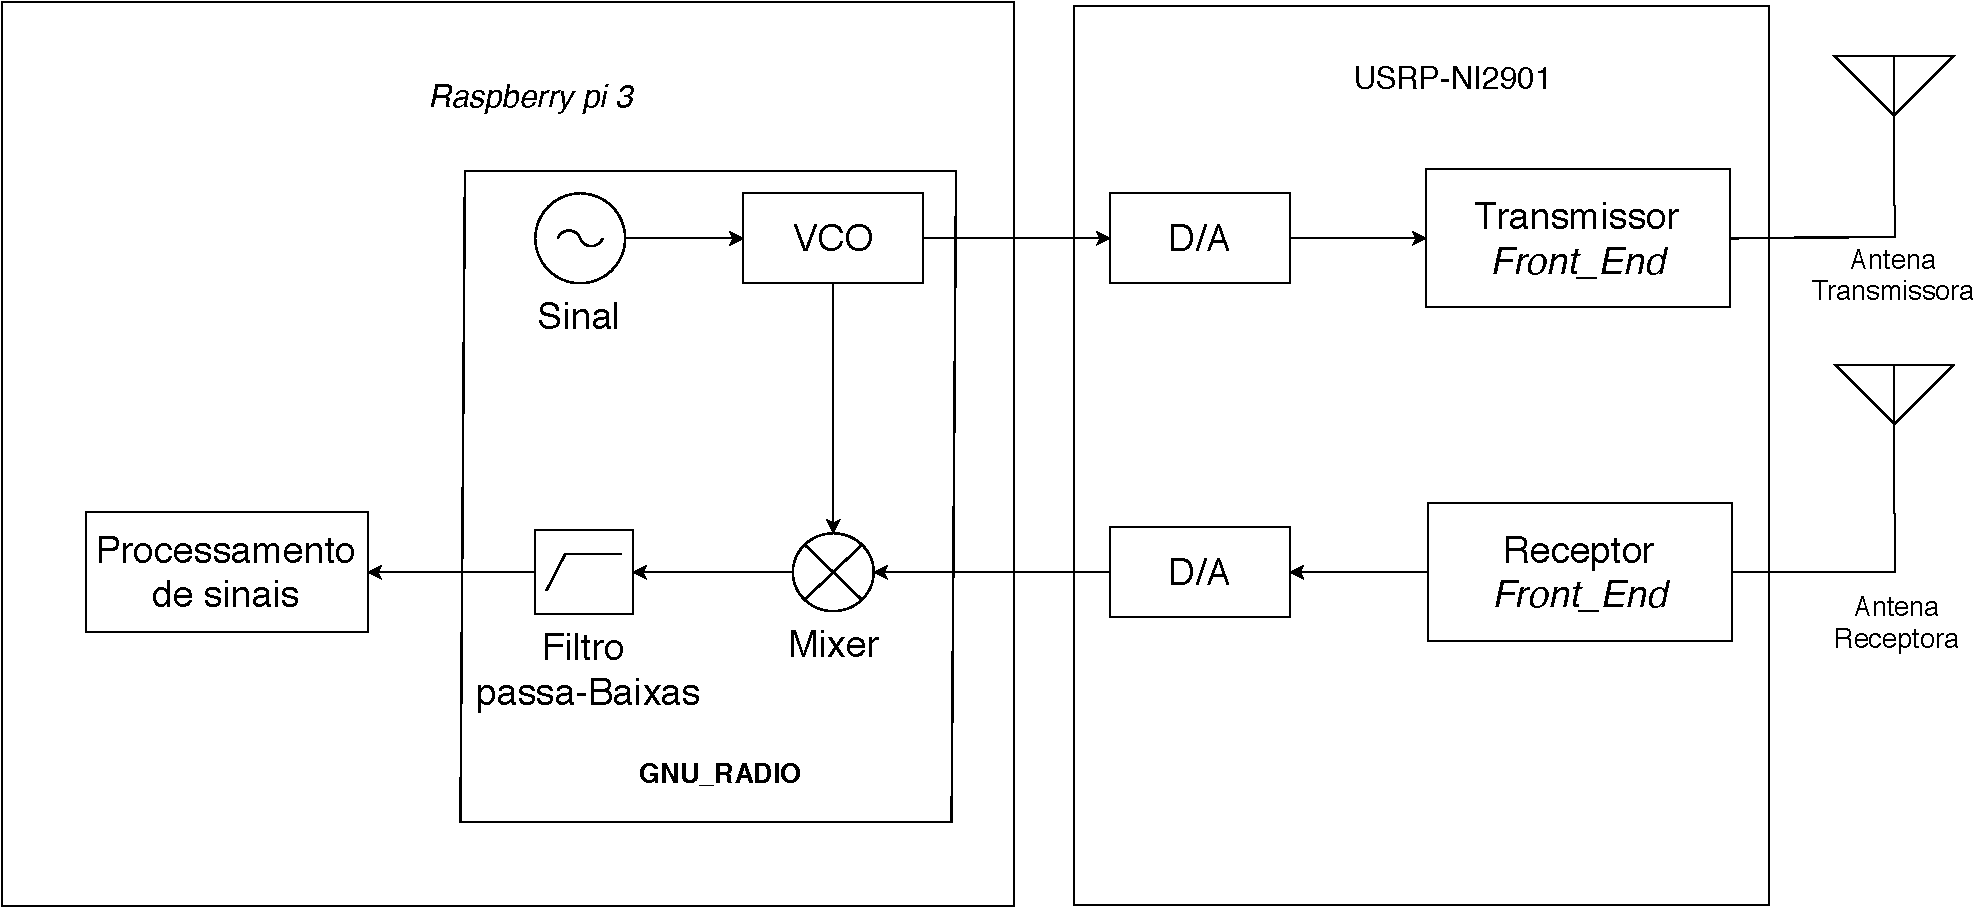
\includegraphics[scale=0.35]{figuras/diagrama_radar2.pdf}
    \caption{Diagrama do radar utilizado na implementação através do software GNU Rádio.}
    \label{processos_geral_radar}
\end{figure}

Foi utilizado o GNU-RADIO um software de código aberto que fornece blocos de processamento de sinais para implementação em RDS. O software foi embarcado em um microcontrolador \emph{Raspberry Pi 3} que através do GNU-RADIO envia e recebe os sinais, após a recepção o sinal é processado no microcontrolador e calculado o desvio de frequência para então ter a velocidade do veículo. 


O sinal da portadora escolhido, de acordo com a Figura \ref{processos_geral_radar}, é modulado no bloco \emph{VCO - Voltage-Controlled Oscillator}, no qual o sinal oscila através de uma frequência central e, de acordo com a sensibilidade do VCO e a amplitude da portadora, variam com o tempo fazendo com que a frequência central seja deslocada. Esses dados são enviados da \emph{Raspberry Pi 3} para o USRP através do protocolo de comunicação UART, onde os dados são convertidos de digital para analógico e executados pelo USRP, que através do bloco \emph{front-end} transmissor envia o sinal para antena. Após o sinal se propagar em espaço livre, ser refletido por um objeto e captado pela antena receptora,  é enviado para o bloco \emph{front-end} receptor e depois convertem os dados de analógico para digital, mandando de volta a \emph{Raspberry Pi 3} para o GNU-RADIO passando por um \emph{mixer} e após uma filtro passa-baixas para pegar o desvio de frequência, por fim, o sinal é tratado para obter o cálculo da velocidade.



A resolução de velocidade depende diretamente da resolução em frequência do sinal após a \emph{Fast Fourier Transform} (FFT), que depende da quantidade de amostras adquiridas e da frequência de amostragem, como demonstrado pela Eq. \ref{resolucao_freq}.
\begin{equation}\label{resolucao_freq}
    \Delta f = \frac{f_{s}}{2\,N}
\end{equation}

Onde N é a quantidade de amostras adquiridas, $f_{s}$ a frequência de amostragem e $\Delta f$ a resolução em frequência. A partir da Eq. \ref{resolucao_freq} definiu-se o parâmetro da frequência de amostragem necessária para garantir uma resolução de 1,7 Hz para uma determinada quantidade de amostras, neste projeto 1024 amostras, resultando em 870 Hz para o sinal a ser enviado.

\subsection{GNU-RADIO}

    Para montagem do módulo responsável pela detecção da velocidade de objetos ao se aproximarem da área de funcionamento do radar, optou-se por utilizar o software \emph{GNU-RADIO} seguindo o diagrama a seguir:

\begin{figure}[H]
    \centering
    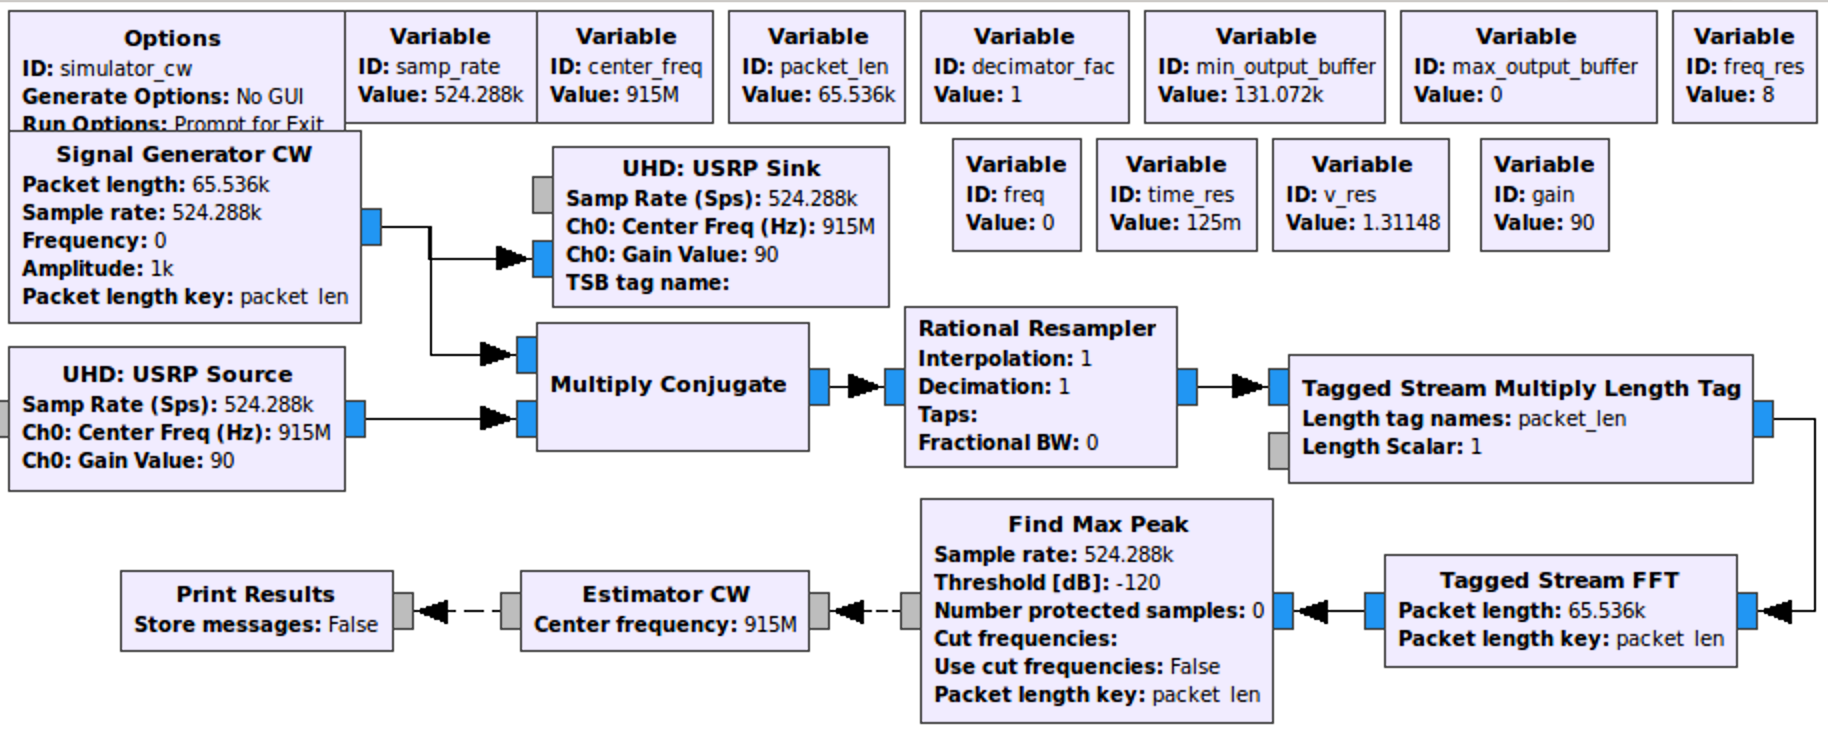
\includegraphics[scale=0.4]{figuras/GNUR.png}
    \caption{Diagrama em blocos da solução do sistema de radar.}
    \label{GNU}
\end{figure}

Onde podemos definir a função de cada um dos blocos da seguinte forma:
\begin{itemize}
    \item \emph{Signal Generator CW}: Este bloco é responsável por gerar o sinal em banda base para ser transmitido pelo \emph{SDR}, sendo que os parâmetros necessários para gerenciar o bloco são \emph{packet len}, \emph{samp rate}, frequência e amplitude;
    \item \emph{UHD: USRP Sink}: Bloco disponibilizado no repositório da empresa do rádio utilizado, de modo que o bloco é responsável por transmitir a mensagem de acordo com a frequência desejada, de modo que seus parâmetros principais são \emph{samp rate}, \emph{Center Frequency}, \emph{Gain} e \emph{Band};
    \item \emph{UHD USRP Source:}  Bloco disponibilizado no repositório da empresa, responsável por realizar a recepção dos sinais através da antenas sendo seus principais parâmetros \emph{samp rate}, \emph{Center Frequency}, \emph{Gain} e \emph{Band};
    \item \emph{Multiply Conjugate}: Responsável por realizar o \emph{downconverter} do sinal que é captado pela antena, possibilitando com que o mesmo seja processado pelo software;
    \item \emph{Rational Resampler}: Realiza uma decimação do sinal amostrado através do qual algumas amostras são descartadas com o intuído de manter uma taxa de dados. 
    \item \emph{Tagged Stream Multiply Leng Tag}: Através do tamanho de cada um dos pacotes de dados obtidos pelo \emph{samp rate} do sinal é transformado em varias tags;
    
    \item\emph{Tagged Stream FFT:} Realiza a FFT janelada das amostras no tempo de modo  a aumentar ou diminuir sua resolução devido ao tamanho do pacote utilizado.
    \item \emph{Find Max Peak:} Pega o espectro do sinal no tempo e com isso realiza uma busca no espectro de modo a encontrar os picos de frequências presentes no espectro do sinal.
    \item \emph{Estimator CW:} Através dos valores dos índices representados pelos picos de frequência de cada amostra e também sabendo qual a frequência do sinal enviado é possível estimar a velocidade dos objetos que se aproximam ou afastam do radar;
    \item \emph{Print Results}: Realiza a captura e armazenamento dos valores obtidos pelo radar com o intuito de ser jogada essas informações para o sistema de controle do radar.
\end{itemize} 

\subsection{Testes e resultados}

    Foram realizados dois testes para validação do sistema do radar. O primeiro teste consistiu em realizar um experimento em campo para captação do movimento de um automóvel através do desvio de frequência da recepção em relação à frequência transmitida, sendo esta última deslocada para zero com o intuito de se visualizar somente sua variação no momento em que o veículo se aproxima a uma distância de 20 metros. O resultado do teste é mostrado na Figura \ref{TVeiculo}.

\begin{figure}[H]
    \centering
    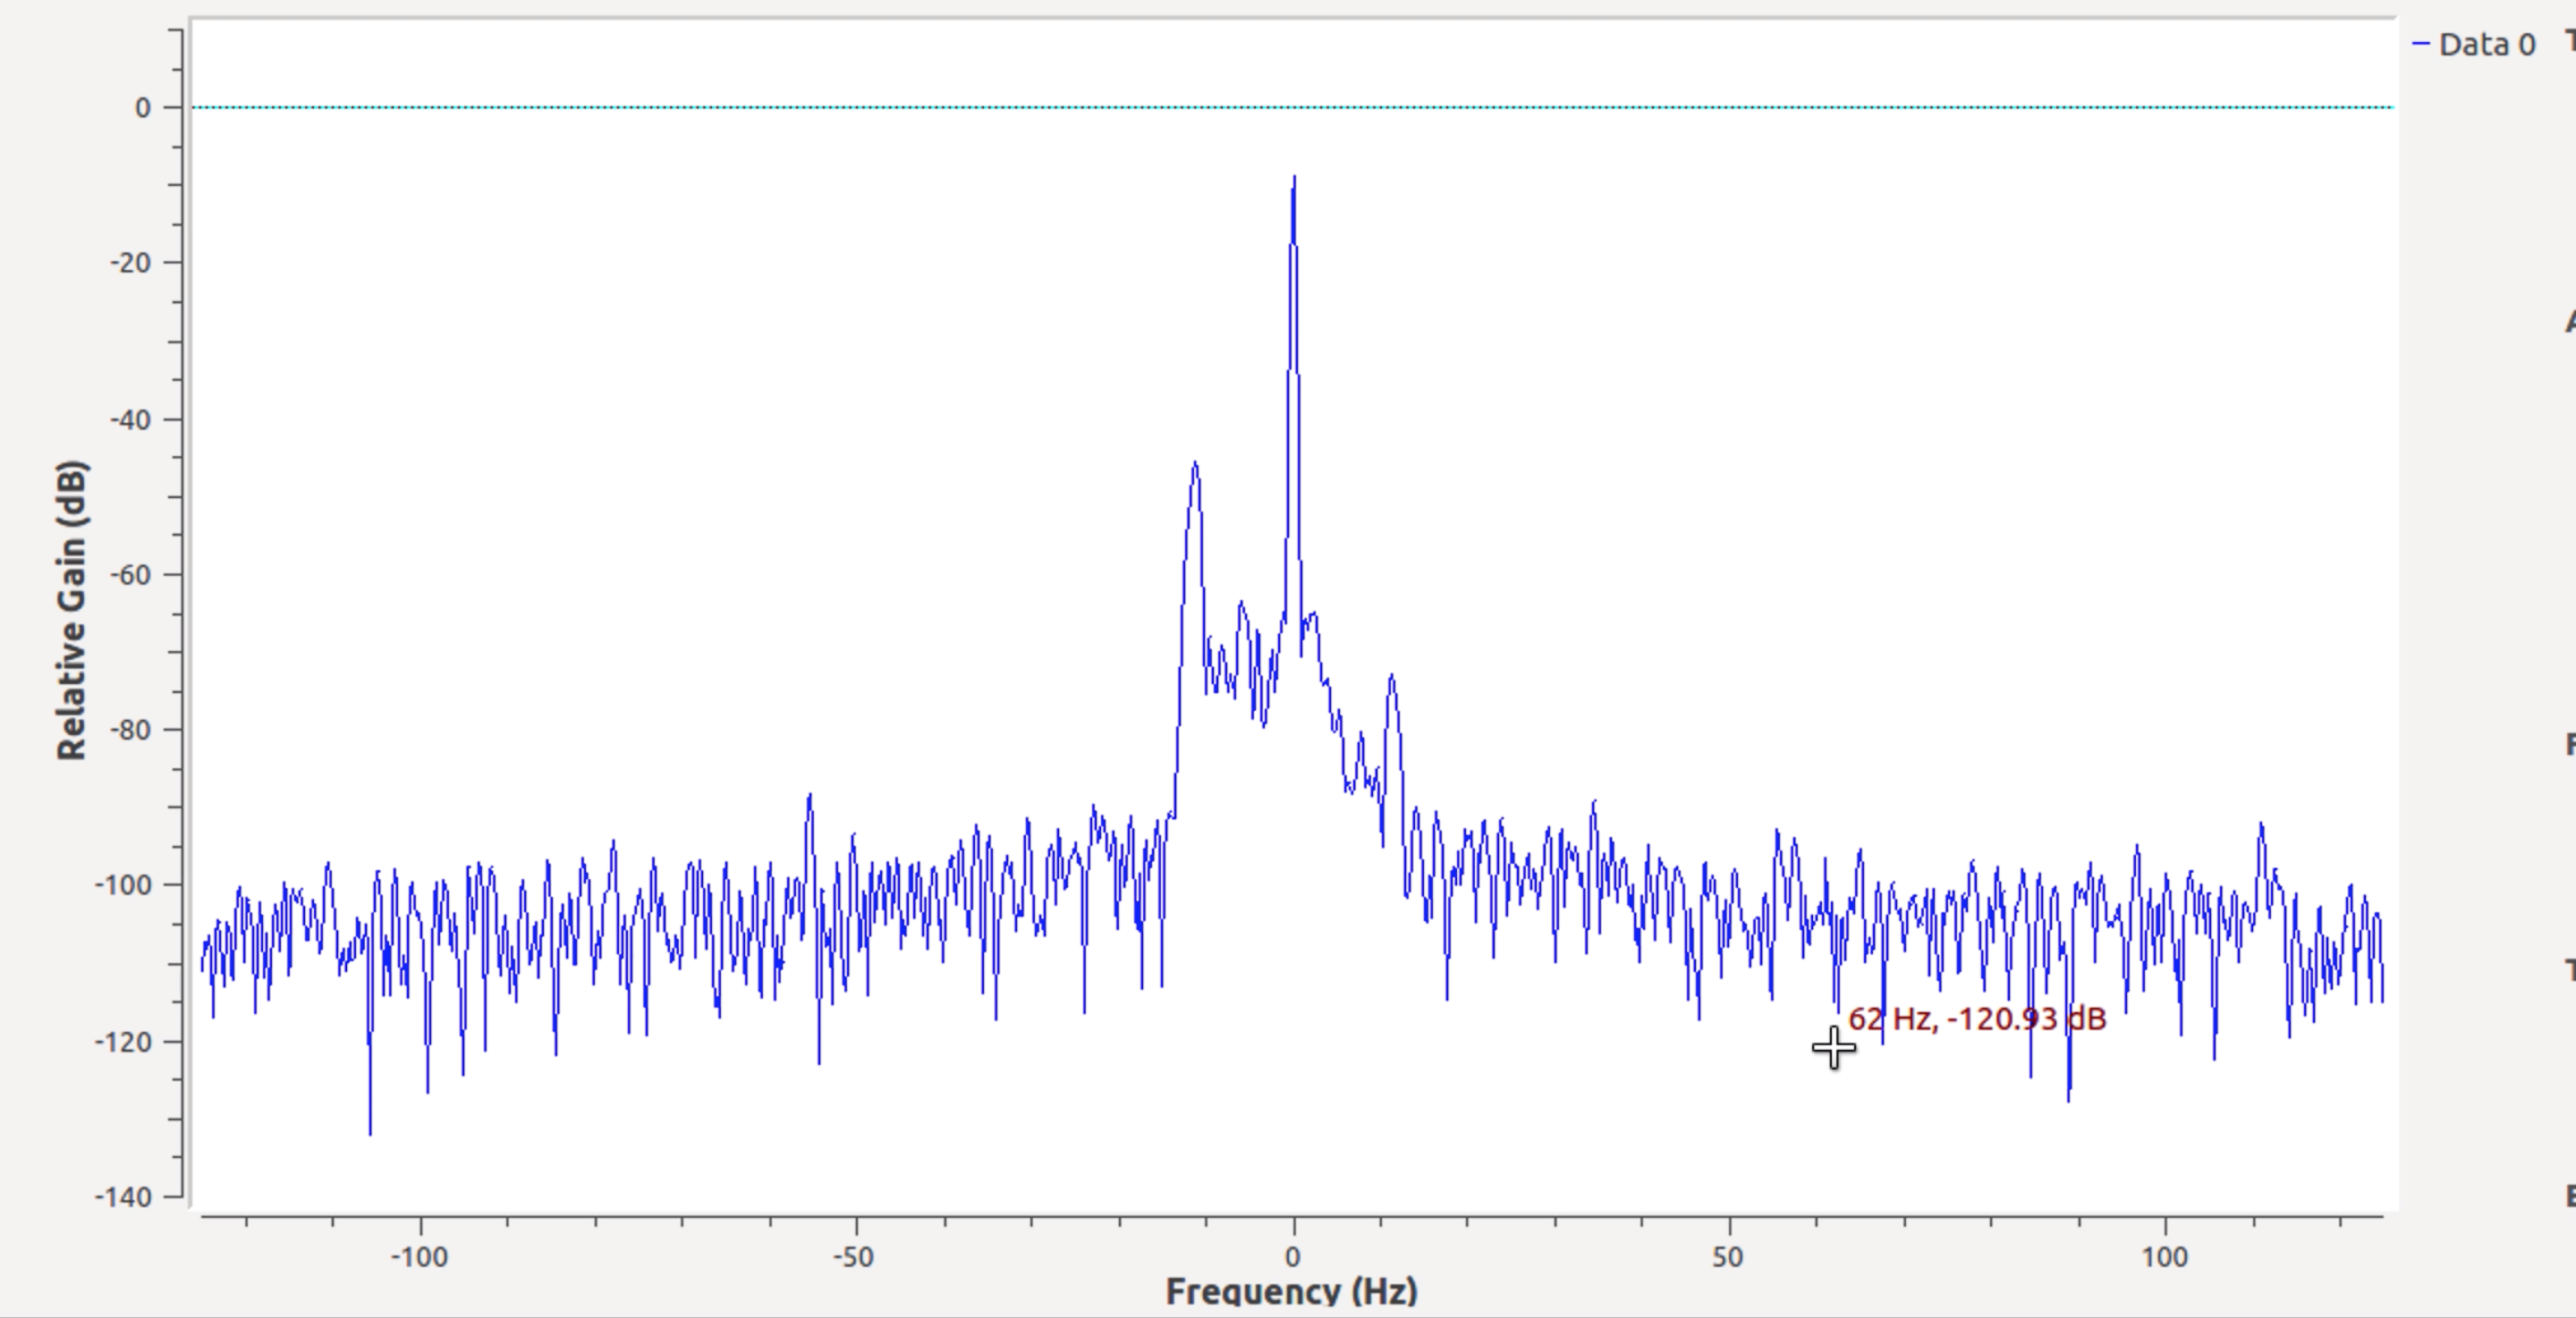
\includegraphics[scale=0.23]{figuras/Carro.png}
    \caption{Gráfico ilustrando o desvio de frequência causado pela captura de um veículo em movimento.}
    \label{TVeiculo}
\end{figure}

A Figura \ref{TVeiculo} mostra a FFT da recepção do sinal no momento o qual o carro se aproxima do radar, onde no centro temos o pico de maior ganho que representa frequência de transmissão de 915MHz na qual a antena está transmitindo, e o pico secundário dentro da FFT representa a o deslocamento em frequência causado pelo movimento do carro, e de acordo com essa variação e utilizando a equação \ref{Doppler} é possível estabelecer a velocidade do mesmo pelo radar.

Com isso foi possível validar a transmissão e recepção do sinal à distância estipulada na seção de cálculos do radar. 

O segundo teste realizado com o radar consistiu em
medir a variação de velocidade radial na qual um sinal refletido por um ventilador é captado pela antena, por se tratar de uma velocidade angular irá aparecer no espectro do sinal várias frequências que estão relacionadas com a velocidade linear do ventilador ao longo da pá do mesmo, como mostrado nas Figuras \ref{fig:velocidade}.

\begin{figure}[H]

    \centering
      \begin{subfigure}{\textwidth}
        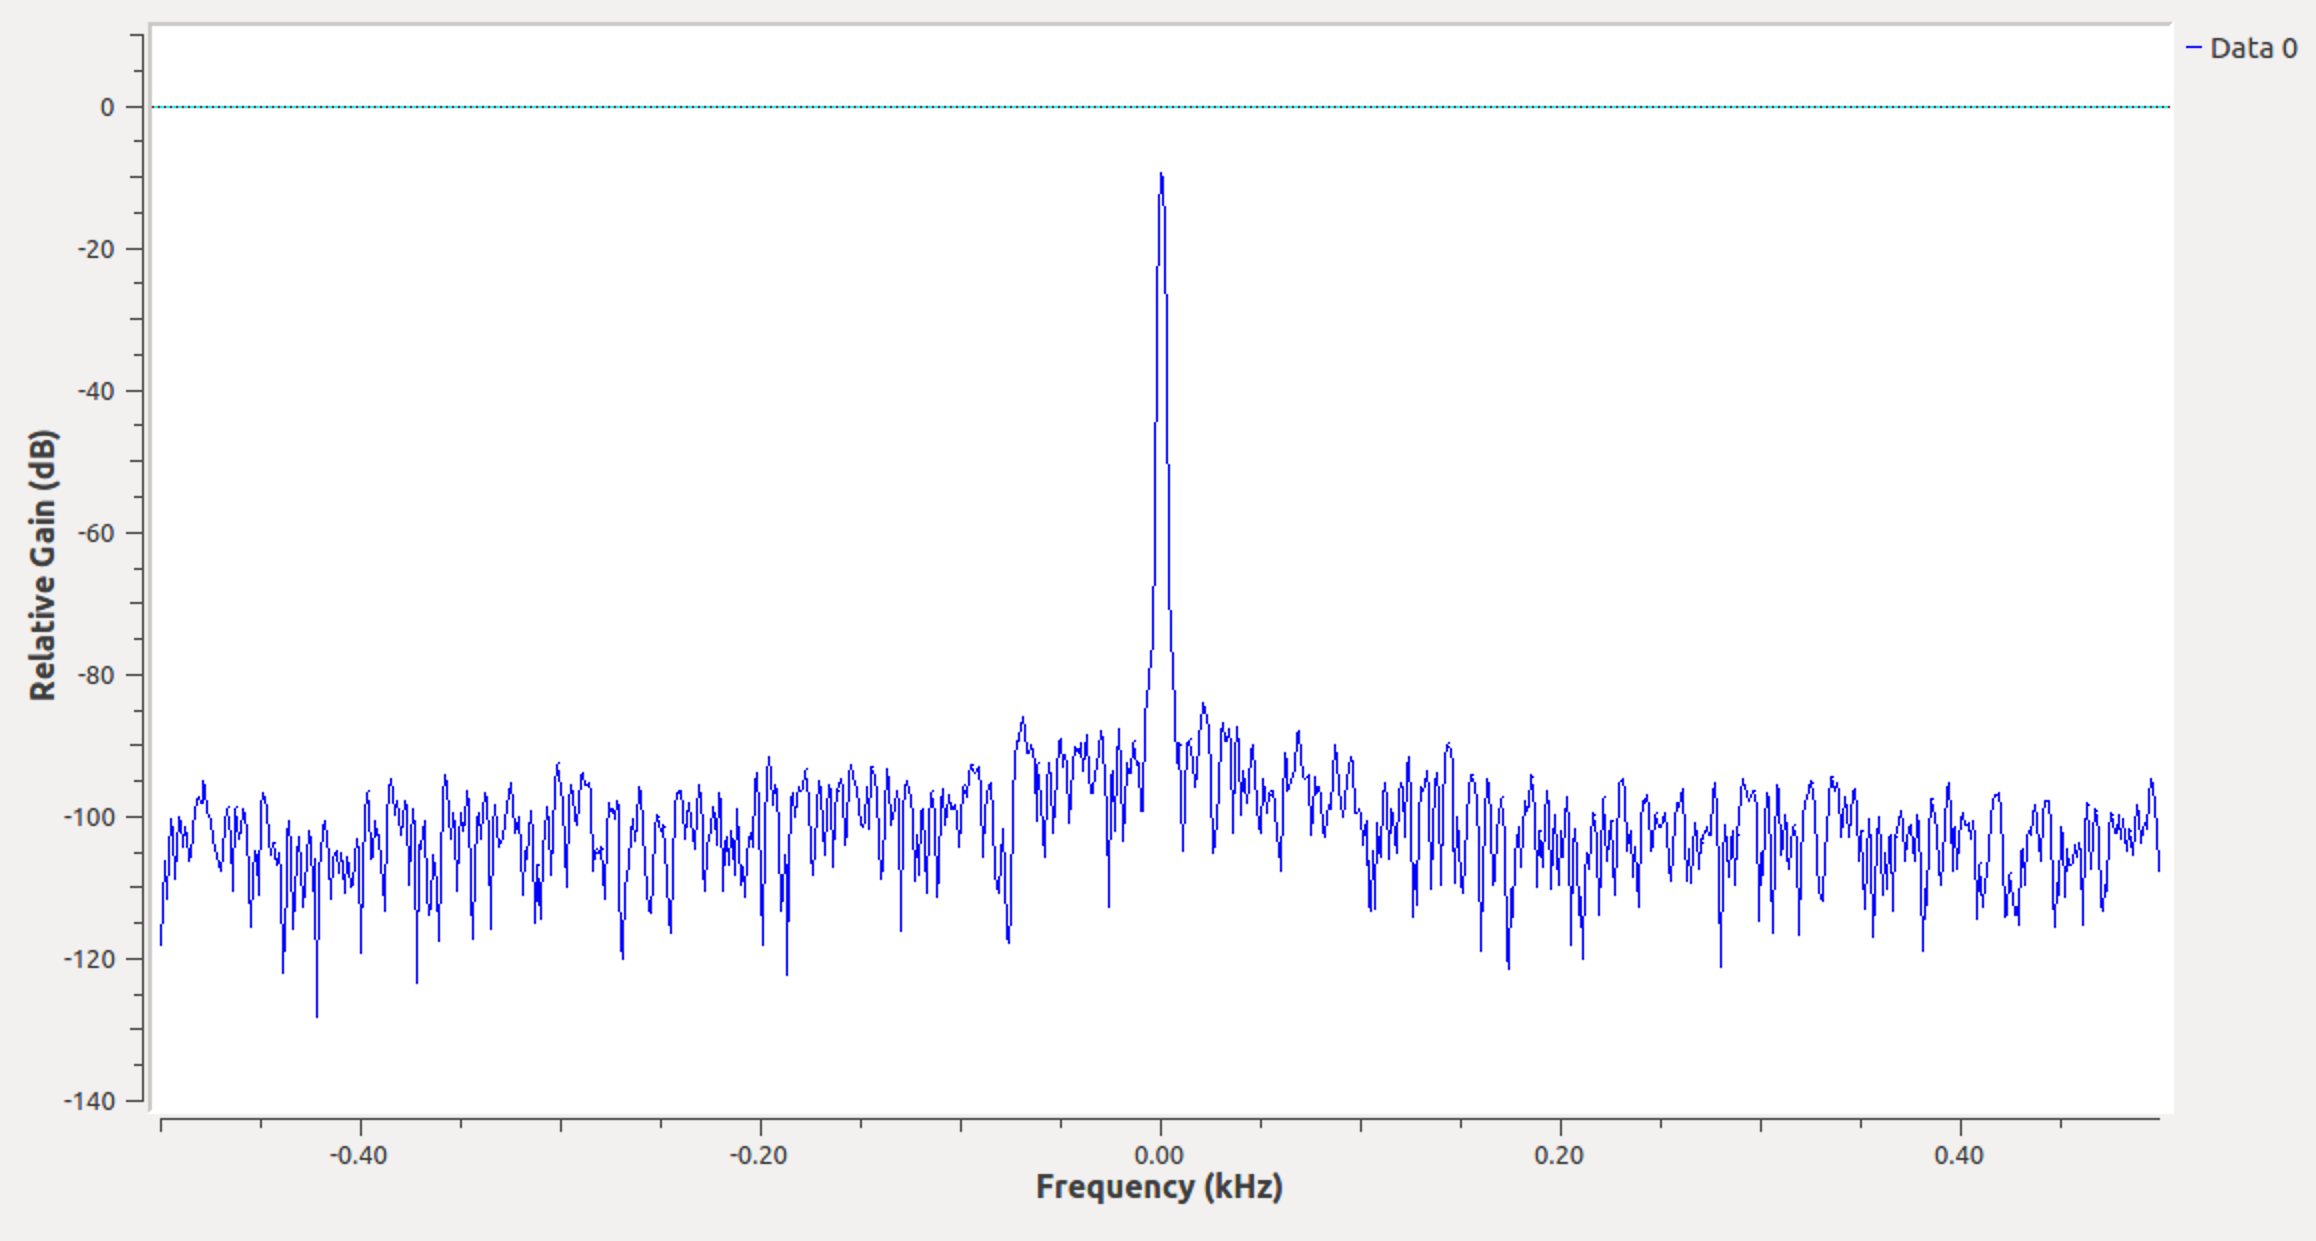
\includegraphics[scale=0.3]{figuras/Ventilador_desligado.png}
    \caption{Imagem da captação do radar com o ventilador desligado.}
    \label{Vel0}
      \end{subfigure}
      \hfill
      \begin{subfigure}{\textwidth}
       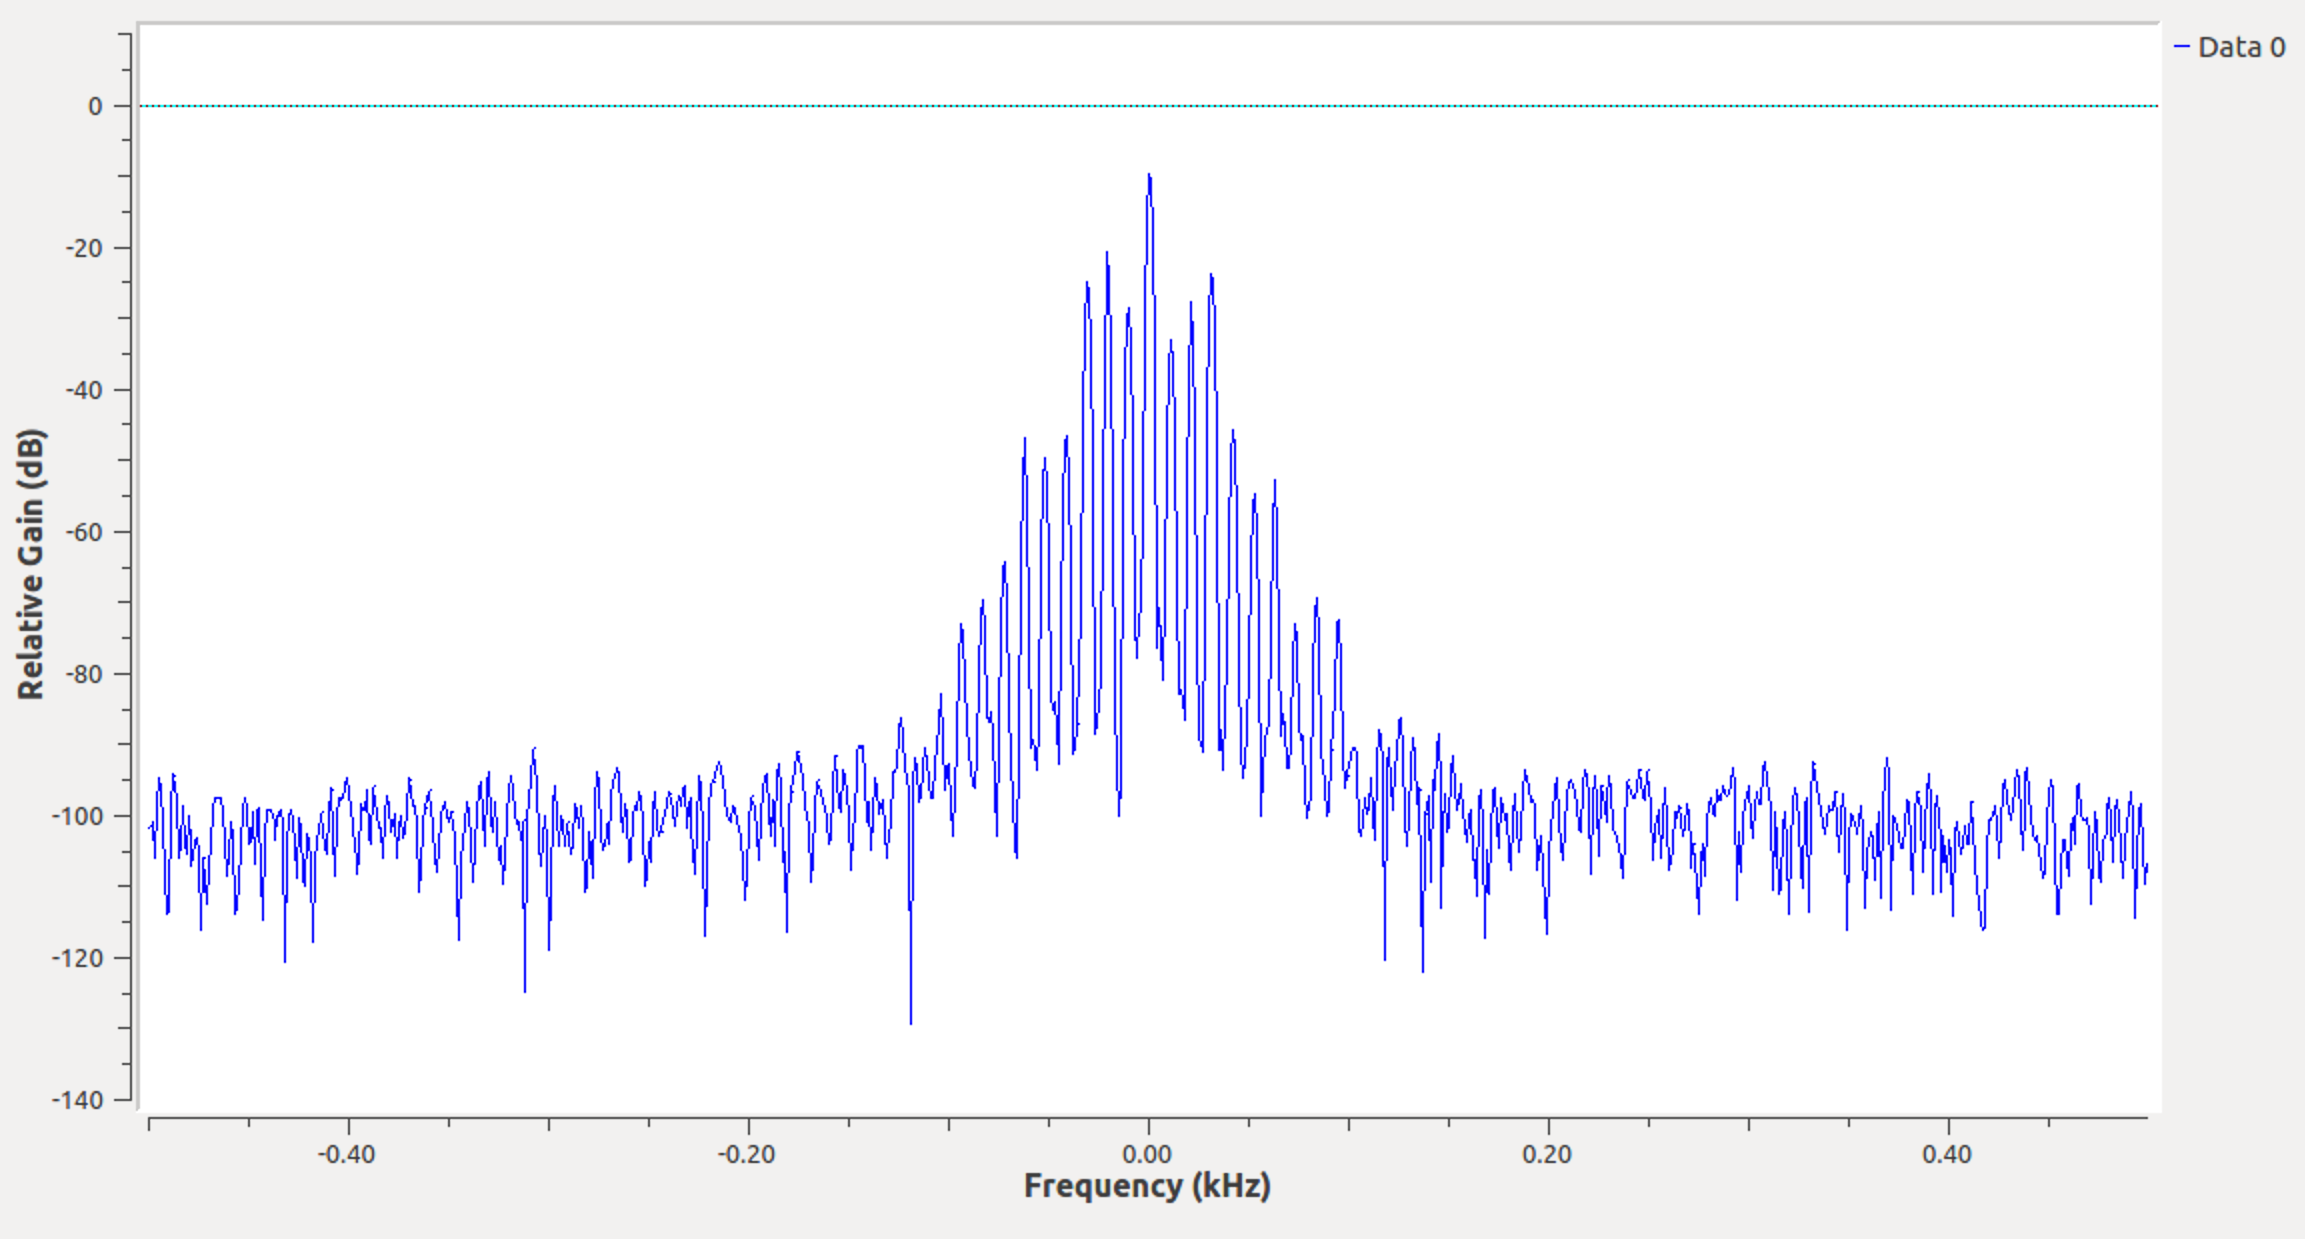
\includegraphics[scale=0.3]{figuras/Ventilador_vel1.png}
    \caption{Imagem da captação do radar em velocidade 1.}
    \label{Vel1}
      \end{subfigure}

\end{figure}

\begin{figure}[H]\ContinuedFloat
    \centering
    \begin{subfigure}{\textwidth}
        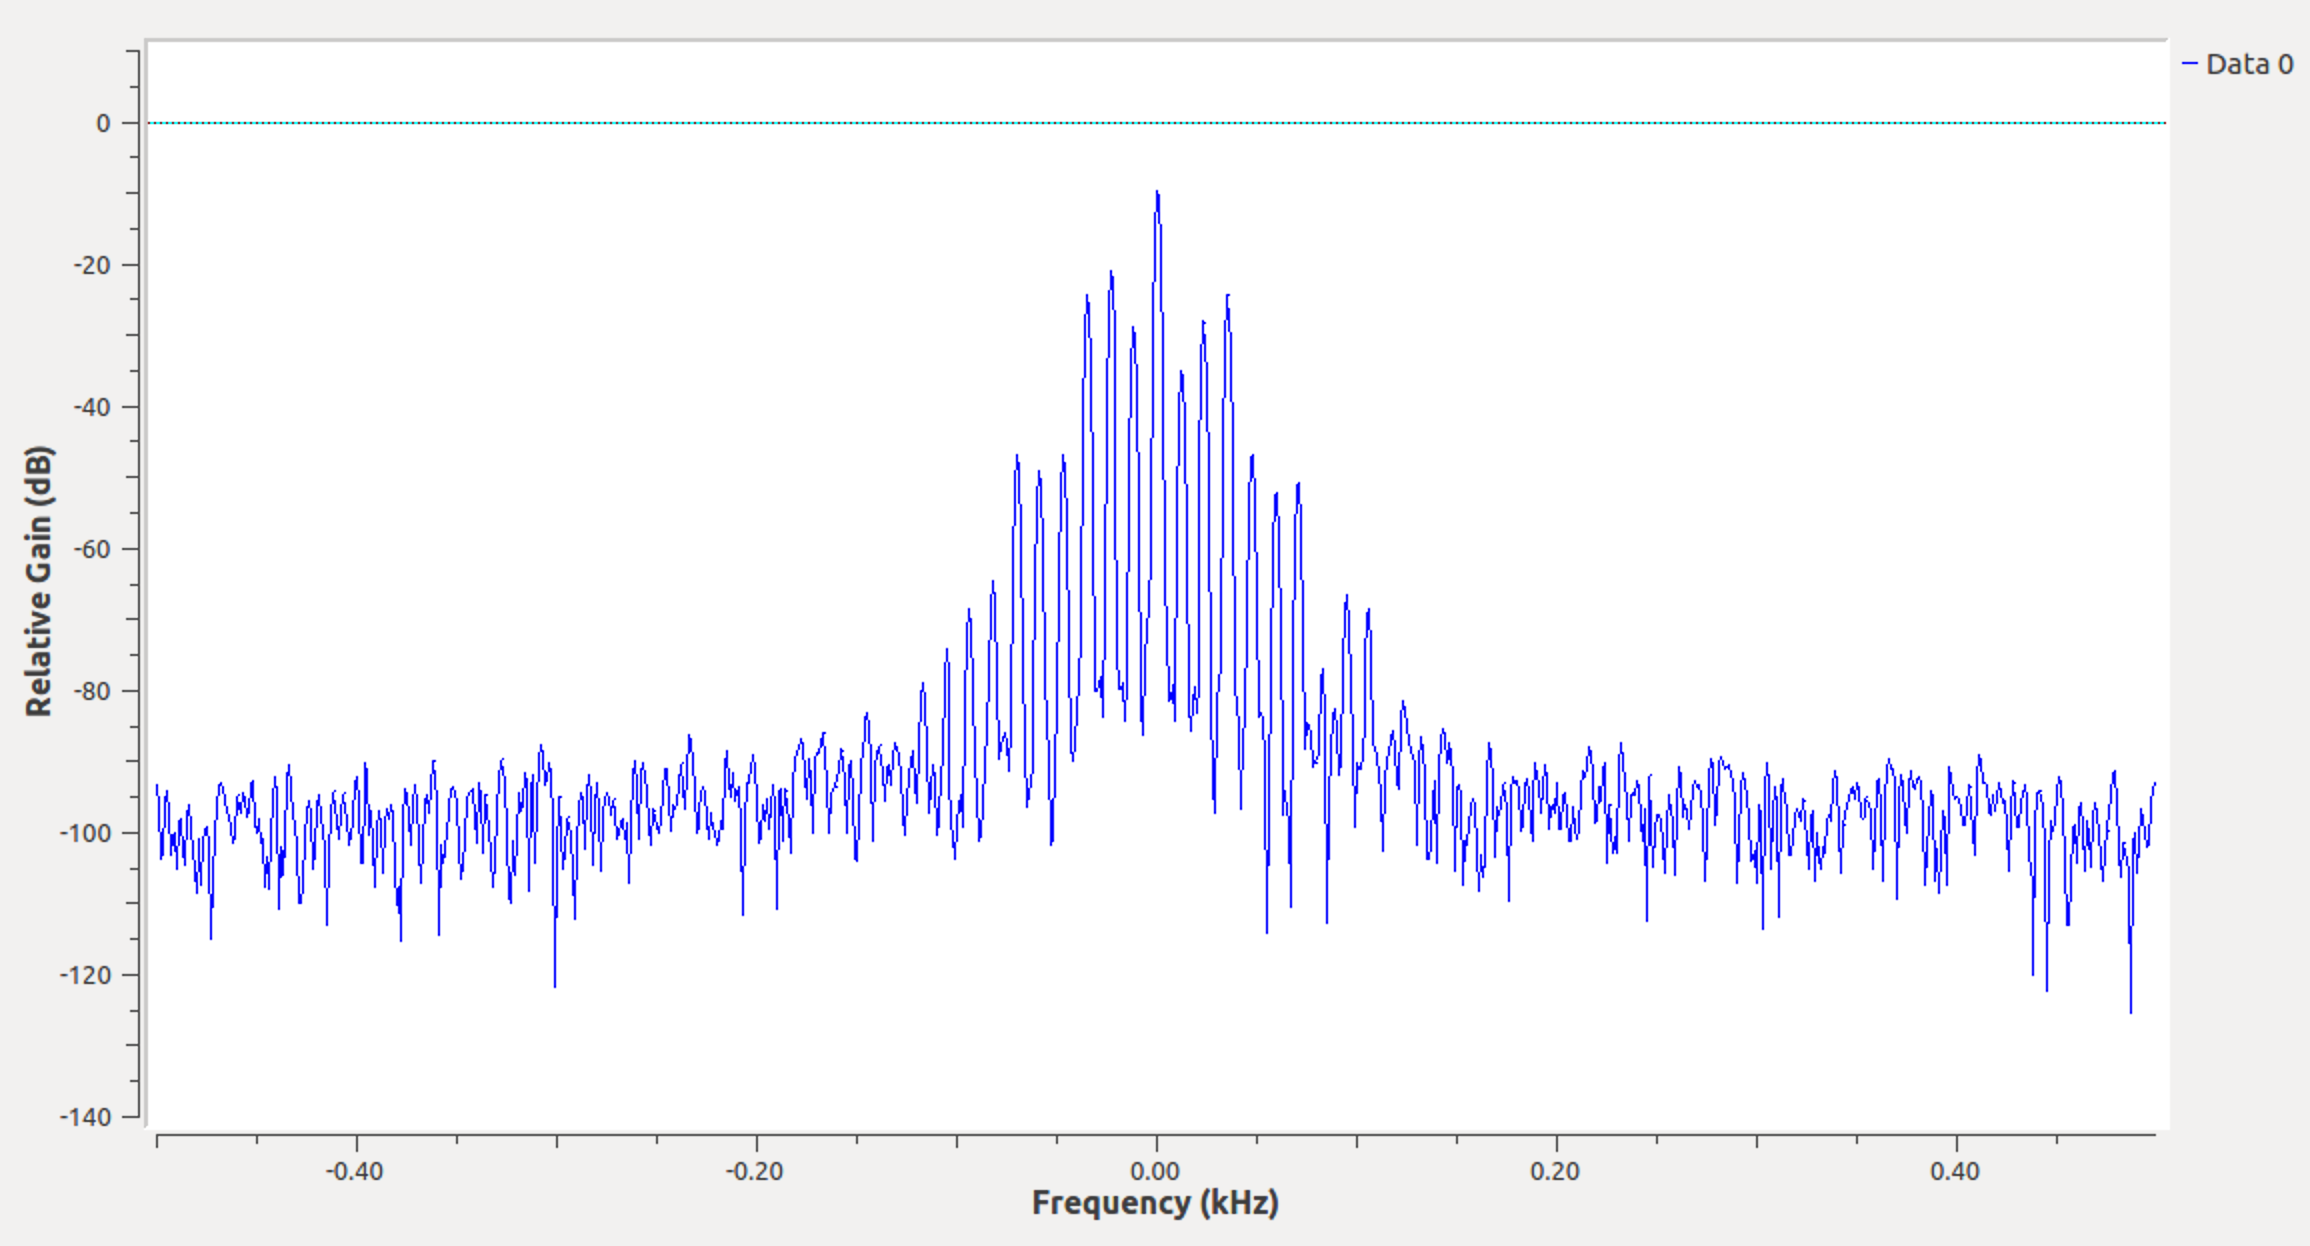
\includegraphics[scale=0.3]{figuras/Ventilador_vel2.png}
    \caption{Imagem da captação do radar em velocidade 2.}
    \label{Vel2}
      \end{subfigure}
\begin{subfigure}{\textwidth}
       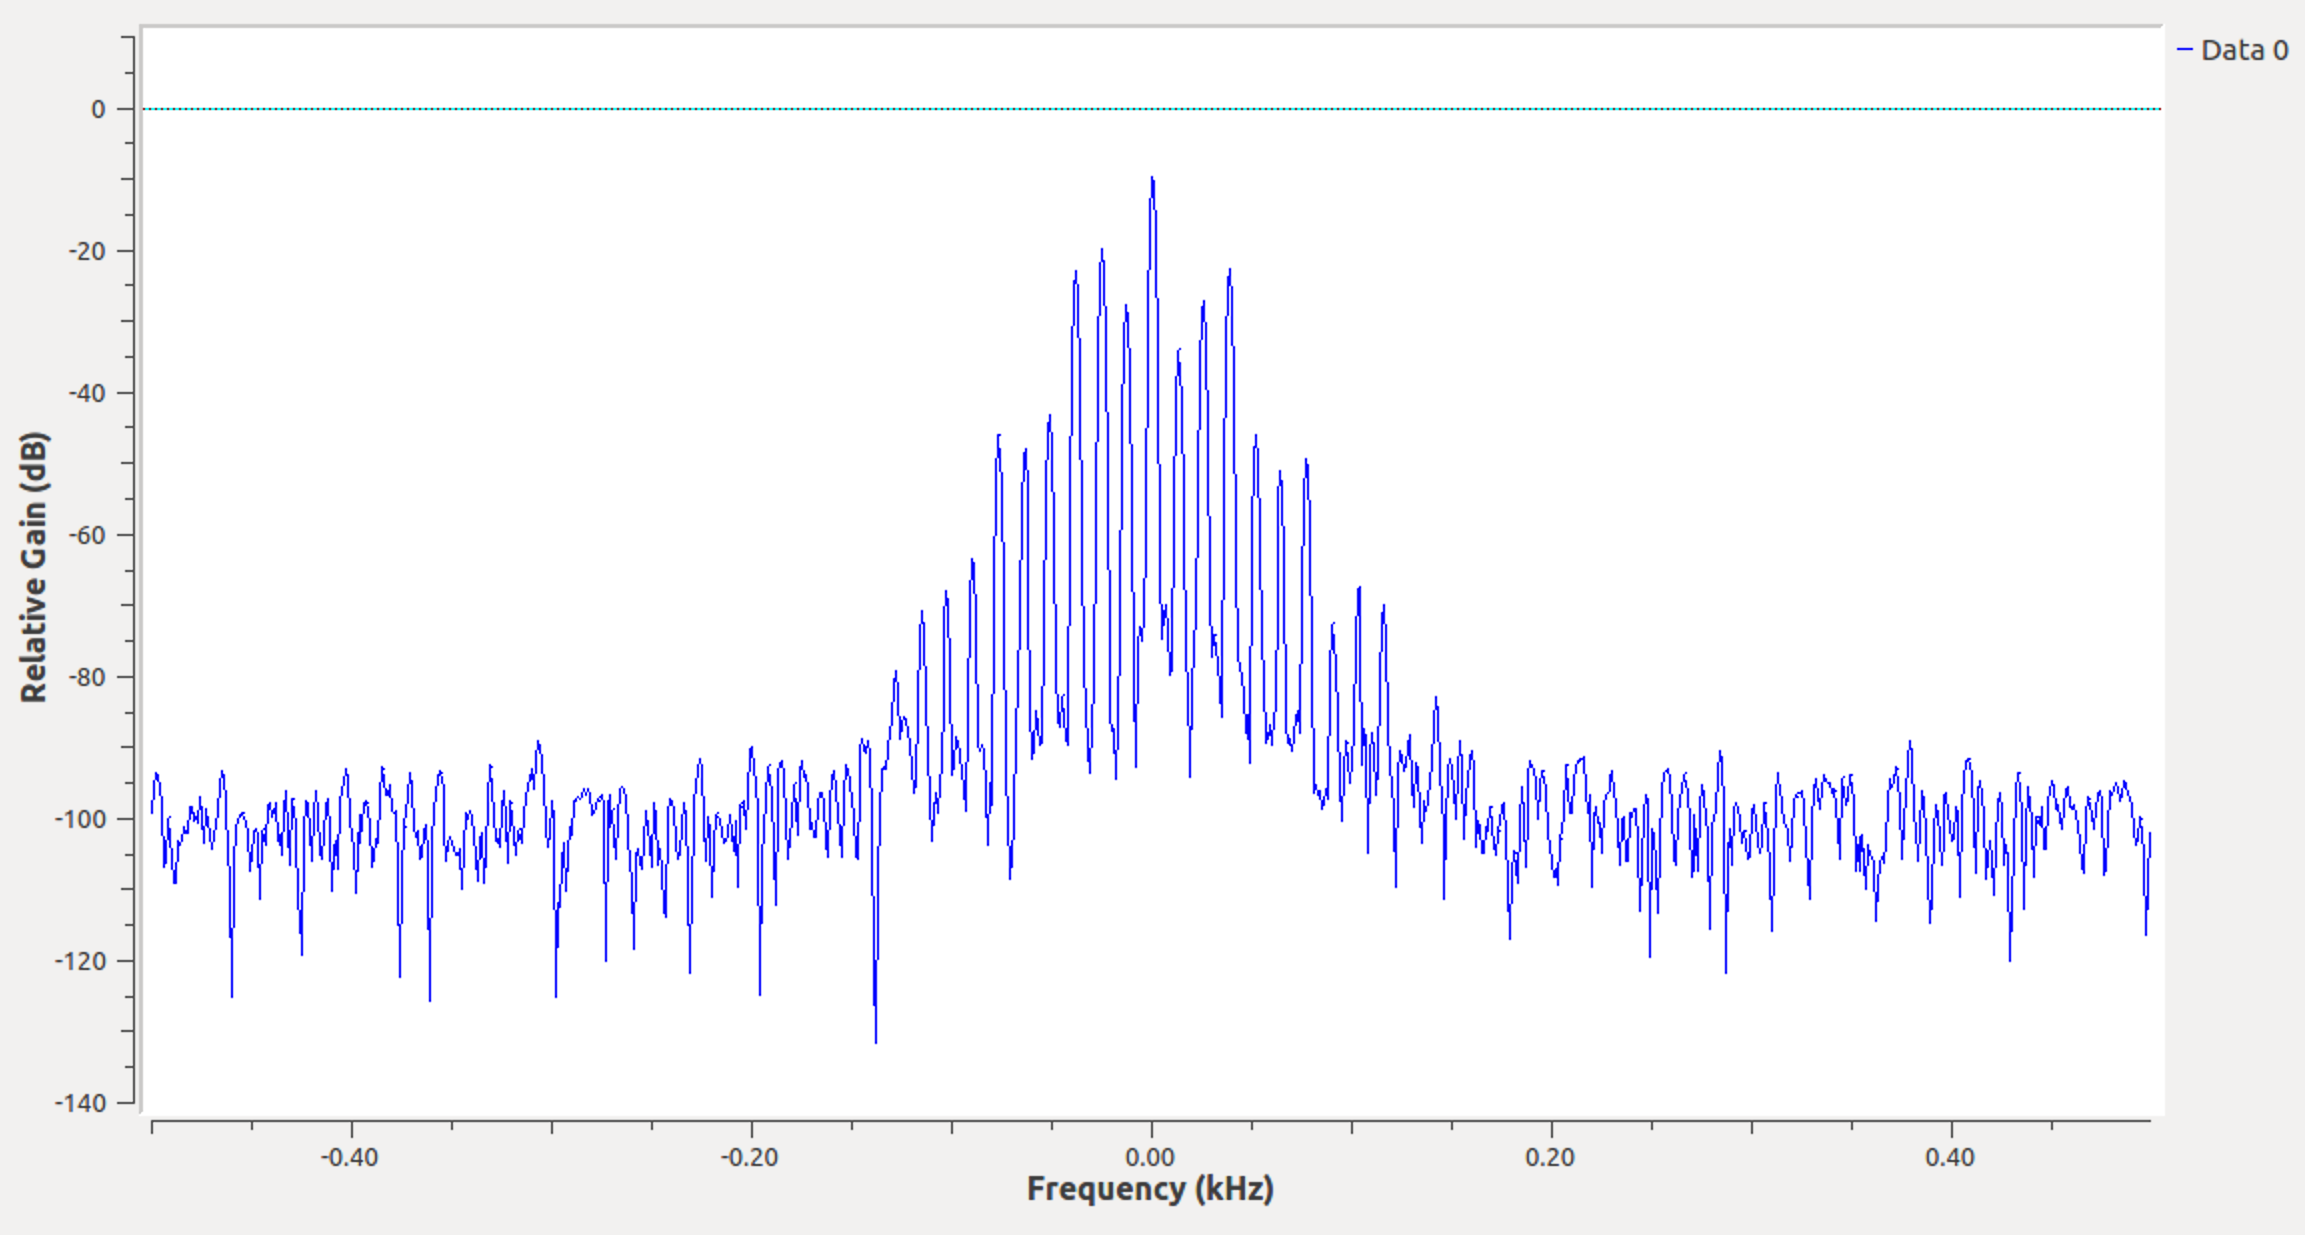
\includegraphics[scale=0.3]{figuras/Ventilador_vel3.png}
    \caption{Imagem da captação do radar em velocidade 3.}
    \label{Vel3}
      \end{subfigure}
      \caption{Captação de diferentes velocidades no radar.}
      \label{fig:velocidade}
\end{figure}
%%%%%%%%%



De acordo com o a Figura \ref{Vel0} onde pode ser verificado somente um pico na frequência de transmissão da antena, concluindo que não ha nenhum objeto com velocidade radial próximo do radar. Já na Figura \ref{Vel1} pode verificar um espalhamento espectral do sinal na recepção, pelo fato de que quando o sinal refletir sobre o ventilador a antena irá captar um grande número de velocidades devido ao aumento gradual da velocidade linear de acordo com que o sinal refletido está mais afastado do centro do ventilador fazendo com que isso seja enxergado como um espalhamento na FFT do sinal na recepção. De acordo como são analisadas as Figuras \ref{Vel2} e \ref{Vel3}, pode-se notar a expansão do espalhamento espectral devido ao aumento da velocidade angular do ventilador.


%%%%%%%%%%%%%%%%%%%%%%%%%%%%%%%%%%%%%%%%%%%%%%%%%%%%%%%%%%%%%%%%%%%%%%%%%%%%%%%%%%%%%%%%%%%%%%%%%%%%%%%%%%%%%%%%%%%%%%%%%%%%%%%%%%%%%%%%%%%%%%%%%%%%%
        
\section{Sistema de controle}

O sistema de controle tem como função principal realizar o processamento de imagens, monitoramento e comunicação dos vários módulos presentes no projeto. Os sistemas foram embarcados em um microprocessador \emph{Raspberry Pi 3}, onde a Figura \ref{redePetri} mostra o diagrama de estados do sistema em rede Petri no software PIPE. A \emph{Raspberry pi 3} foi escolhida pelo seu alto desempenho com relação ao tempo de processamento dos sinais que são enviados, por atender a todos os protocolos de comunicação a serem feitos com os módulos escolhidos e também por apresentar um bom custo-beneficio.

\begin{figure}[H]
    \centering
    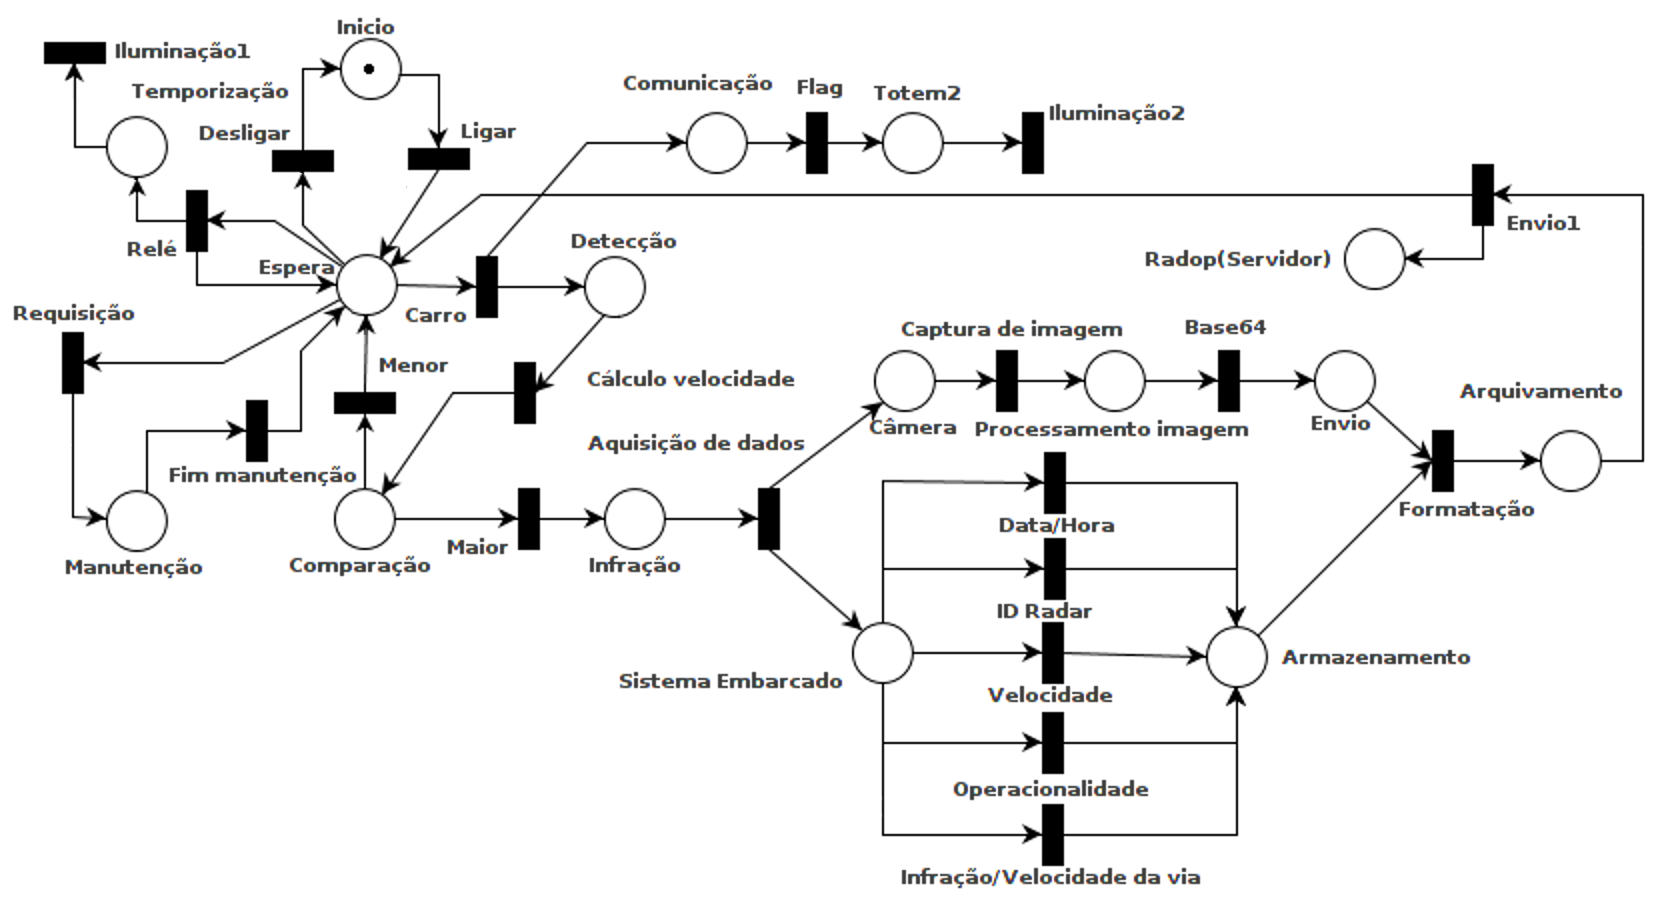
\includegraphics[scale=0.4]{figuras/Petri.png}
    \caption{Rede de Petri para a solução proposta para o sistema eletrônico, feito no software PIPE.}
    \label{redePetri}
\end{figure}

A Figura \ref{comunicacao} mostra o diagrama de conexão dos diferentes módulos do projeto ligados ao microcontrolador \emph{Raspberry Pi 3}, além disso mostra as alimentações e os protocolos de comunicação utilizados por cada um dos componentes. A linguagem de programação utilizada para o funcionamento do sistema de controle foi o \emph{Python}. Foi utilizado várias \emph{threads} para que algumas funções fossem executadas em paralelo para uma não atrapalhar na outra.

     \begin{figure}[H]
    \centering
   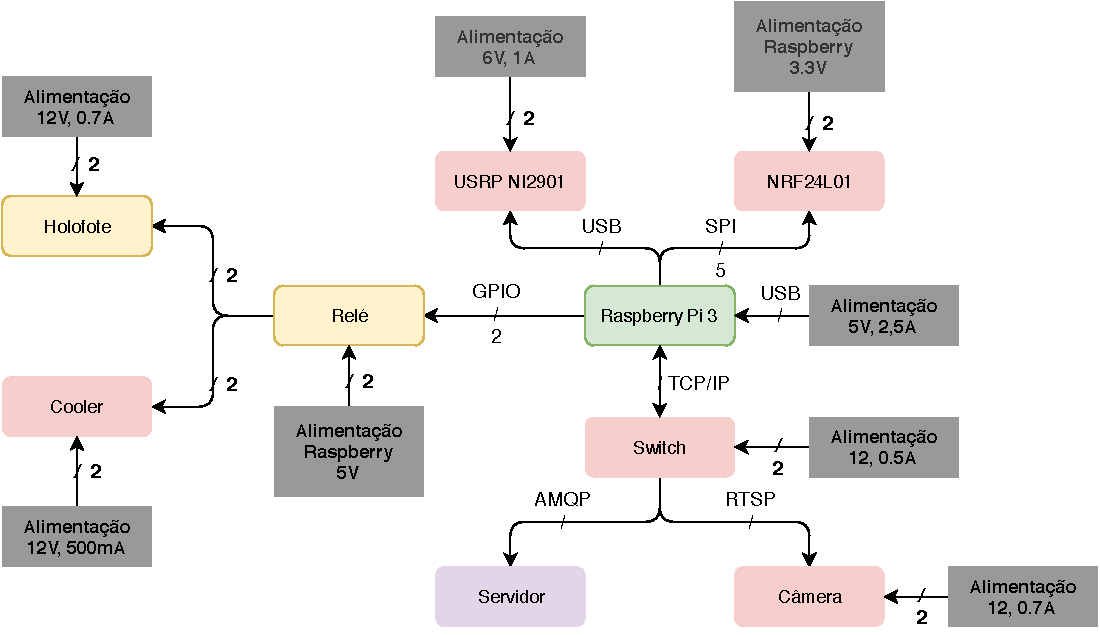
\includegraphics[scale = 0.6]{figuras/Diagram_Geral.pdf}
   \caption{Diagrama lógico do sistema de controle do projeto, onde o microprocessador \emph{Raspberry Pi 3} controla os demais sistemas e faz as comunicações. Dentre as comunicações estão o servidor, o sistema de sinalização, o sistema de comunicação entre os totens, o controle de captura de imagem com a câmera, o pré-processamento da imagem e o \textit{cooler}. Feito no \emph{software Draw.io}.}
   \label{comunicacao}
    \end{figure}
    

\subsection{Tempo de latência}\label{tempo_latencia}

Dentre os principais requisitos solicitados pelo microprocessador é que deve possuir uma latência máxima de operação para se comunicar entre os módulos de aproximadamente 1.36 segundos, sendo este dado obtido através do tempo em que um veículo com velocidade máxima de 150 km/h usaria para percorrer a distância do ponto de captura de sua velocidade, no máximo a 50 metros antes do radar, até o ponto onde ocorre a captura da imagem, a 7 metros após o radar, caso ocorra uma infração. 
      
\subsection{Sinalização}
    
Quando o veículo se aproxima do radar, é enviada uma informação para o outro totem, que aciona um aviso luminoso alertando o condutor que um automóvel se aproxima em direção oposta, e que os mesmos redobrem a atenção realizando a curva ao mesmo tempo. 

Para este processo foram utilizados o módulo \emph{Wi-fi} NRF24L01, um relé de 5V e um holofote. O NRF24 foi utilizado tanto para transmitir a \emph{flag} para o outro radar, quando ocorre detecção de um veículo, quanto para recepção da \emph{flag} que vem do outro totem, quando é verificado uma detecção no outro radar. No momento em que o módulo NRF24 recebe uma \emph {flag}, o sistema de controle envia um sinal para o relé que faz o chaveamento para ligar o aviso luminoso por 5 segundos, sendo que o mesmo é atualizado quando detectado outro carro durante este intervalo de tempo, alertando o condutor sobre um veículo se aproximando na direção contrária. Esse tempo de 5 s de iluminação é necessário pelo fato do tempo em que o veículo leva para ser detectado até passar pela curva, usando o pior caso do veículo a 150 km/h em uma curva de 100 m.
A Figura \ref{esquematico} mostra o esquemático do sistema de sinalização, onde são feitas as conexões entre o módulo \emph{NRF24L01}, a \emph{Raspberry Pi 3} e o relé que ligará o holofote.

\begin{figure}[H]
    \centering
    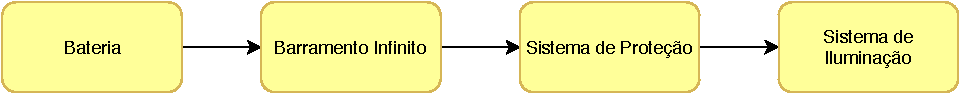
\includegraphics[scale = 0.8]{figuras/esquematico.pdf}
    \caption{Esquemático do sistema de sinalização do radar, que é composto pelo o módulo \emph{NRF24L01} a \emph{Raspberry Pi} e o relé, onde o módulo recebe e transmite o sinal com o outro totem e o microprocessador que aciona através do relé o holofote para fazer a sinalização. Foi utilizado a ferramenta \emph{fritzing}.}
    \label{esquematico}
\end{figure}
   
O protocolo que faz a comunicação entre a \emph{Raspberry Pi} e o módulo NRF24L01 é o \emph{Serial Peripheral Interface} (SPI). Este módulo foi escolhido por ter um baixo consumo de energia, um alcance de sinal de 1 km de distância com outro totem e por sua taxa máxima de 2Mbps, sendo esta velocidade satisfatória em relação a outros protocolos de comunicação. Em relação ao relé sua comunicação com a \emph{Raspberry Pi 3} é por \emph{General Porpouse Input/Output} (GPIO), que são portas de entradas e saídas digitas.  \par
Para execução do código de sinalização foi criado uma \emph{thread}, fazendo com que este processo funcionasse em paralelo com os demais. Para um fácil entendimento deste sistema no código, foi feito uma rede de Petri, mostrada na Figura \ref{Petrisinaliza}.

\begin{figure}[H]
    \centering
    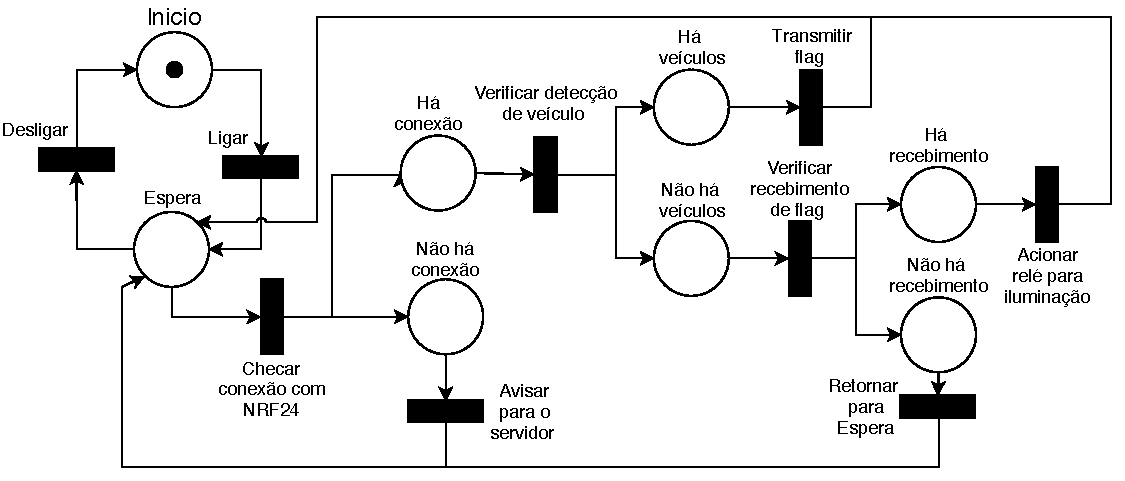
\includegraphics[scale = 0.6]{figuras/sinaliza.pdf}
    \caption{Rede de Petri que representa a \emph{thread} executada no código de controle referente à sinalização. Feito no \emph{software Draw.io}.}
    \label{Petrisinaliza}
\end{figure}. 

Como visto na Figura \ref{Petrisinaliza}, o código irá sempre estar em \emph{loop}. Inicialmente ele verifica se a Raspberry Pi 3 e o módulo \emph{Wi-fi} estão corretamente conectados, para envio de seu \emph{status} posteriormente para o servidor. Já que o módulo NRF24 é \emph{half-duplex}, ele não pode transmitir e receber ao mesmo tempo, e com isso ele fica no modo receber praticamente o tempo inteiro, fazendo uma transmissão apenas ao detectar o carro, e rapidamente volta ao modo receber para que nenhuma comunicação com o outro radar seja perdida. Quando um sinal é recebido do outro totem, é enviado um sinal para o canal 1 do relé através de uma \emph{thread}, fazendo com que a função de detecção continuasse em paralelo ao mesmo tempo que o holofote é ativado pelos 5 segundos, pois caso um carro passe durante este período, uma variável cria uma fila, e antes do holofote ser desligado, é comparado se essa variável possui o mesmo valor antes e depois do tempo ligado. Caso o valor seja igual, significa que nenhum carro passou naquele momento, sendo o holofote desligado. Já se o valor for diferente, significa que outro carro foi detectado, fazendo com o que o holofote seja acrescentado mais 5 segundos ligados até a fila estar com o mesmo valor durante o ultimo incremento de tempo.

\subsection{Controle de Infração}
  
De acordo com o Artigo $5^{\circ}$ Parágrafo $1^{\circ}$ da Resolução do CONTRAN 396/11 \cite{conatran}, a velocidade a ser considerada para que a penalidade seja efetivada é o resultado de uma subtração da velocidade medida pelo equipamento pelo erro máximo admitido previsto na legislação metrológica em vigor, também presente na Resolução \cite{conatran}.
   
 No código, após receber a velocidade do veículo calculada pelo sistema do radar, é encontrada o valor da velocidade considerada, fazendo uma comparação para saber se o veículo realmente está acima da velocidade da via, e se estiver, calculada-se a porcentagem acima da velocidade da via para saber qual tipo de infração o condutor está cometendo, que de acordo com o Artigo 218 do Código de Trânsito Brasileiro (CTB) \cite{ctb} temos 3 (três) tipos de infração, sendo elas a infração média, onde o veículo está no máximo acima 20\%, grave quando o veículo está entre 20 a 50\% e gravíssima quando o mesmo estiver acima dos 50\%.   
A rede de Petri que mostra o processo dentro do sistema de controle se encontra na Seção \ref{Captura}, pois estão funcionando na mesma \emph{thread}.
    

\subsection{Captura}\label{Captura}
    
Caso o veículo detectado esteja acima da velocidade permitida, é realizado uma estimativa de tempo considerando a posição e a velocidade do veículo, que determina quanto tempo o mesmo leva para chegar na região de captura da câmera, realizando o disparo da traseira do veículo.
Primeiramente foi determinado distância de captura de imagem que é entre 10 a 15 metros do radar para realização da captura da imagem. Após, foi levantado os fatores determinantes para uma boa qualidade de imagem para detecção e reconhecimento da placa na distância determinada, sendo o tamanho da lente e também o diâmetro do sensor utilizado pelo aparelho, pois eles influenciam no ângulo de abertura da câmera, e como a distância de captura é considerável, quanto menor for o ângulo de abertura maior é a resolução da imagem captada. Outro fator importante é a utilização de uma lente varifocal, pois esta possibilita um ajuste automático do foco da lente de acordo com que os objetos se aproximam ou afastam dela. Com isso foi escolhido a câmera \emph{Hilook IPC-B620H-V/Z}, com captura de 2 MP e resolução de vídeo máxima de 1920 $\times$ 1280 a 30 fps. \par 
Para realização dos testes a câmera foi configurada com uma qualidade de 1280 x 980 \emph{pixels}, contendo uma qualidade boa e um tamanho de imagem menor em relação a qualidade máxima. Também foi utilizado uma quantidade alta de zoom para diminuir a quantidade de informação desnecessária da imagem e ter uma melhor visualização da placa do veículo, e por último também foi configurado em escala de cinza, diminuindo também o tamanho da imagem. 
\par
Utilizando a biblioteca \emph{OpenCV} e o protocolo de comunicação  \emph{Real Time Streaming Protocol} (RTSP) da pilha de protocolos \emph{Transmission Control Protocol/Internet Protocol} (TCP/IP), foi possível o acesso à câmera para realização da captura, como mostrado na Figura \ref{carro1} com o carro em uma velocidade em torno de 20 km/h. Para a conexão da câmera com a \emph{Raspberry Pi 3} foi utilizado um roteador com rede local, pelo fato da necessidade de ter uma alta taxa de transmissão devido ao envio de imagens para o servidor e da câmera necessitar de uma conexão estável com uma rede para estabelecer uma transmissão contínua. 

%A câmera foi instalada simulando sua posição na estrutura do radar, sendo a 3 metros de altura e a 10 metros de distância da região de captura. 

\begin{figure}[H]
    \centering
    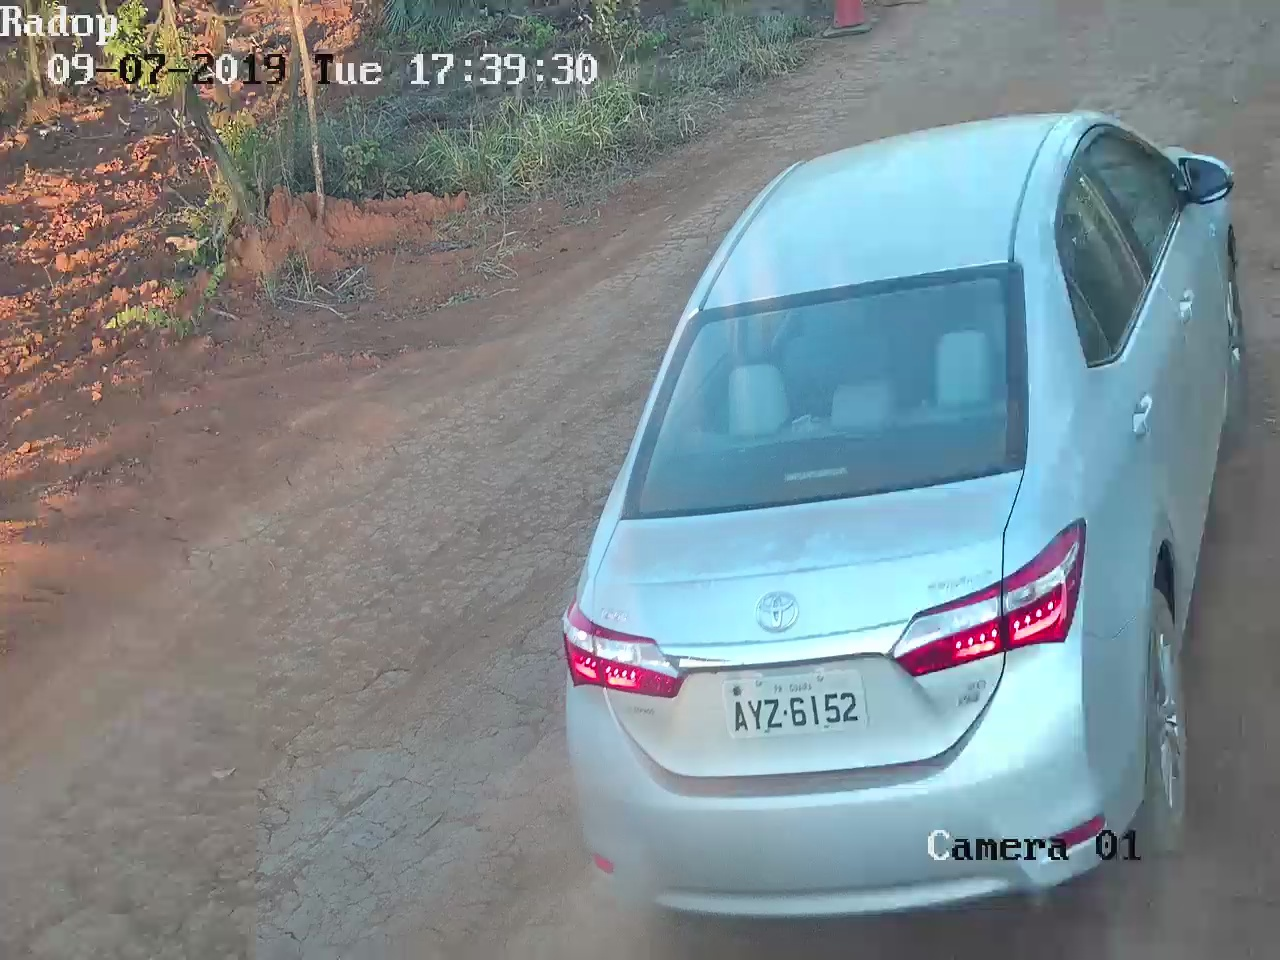
\includegraphics[scale=0.18]{figuras/17_39_34_790981.jpg}
    \caption{Imagem capturada pela câmera no caso de infração do veículo.}
    \label{carro1}
\end{figure}

O processo que realiza tanto a parte de infração quanto de captura em paralelo com as demais está mostrada na rede de Petri na{Figura \ref{Petricaptura}}.

\begin{figure}[H]
    \centering
    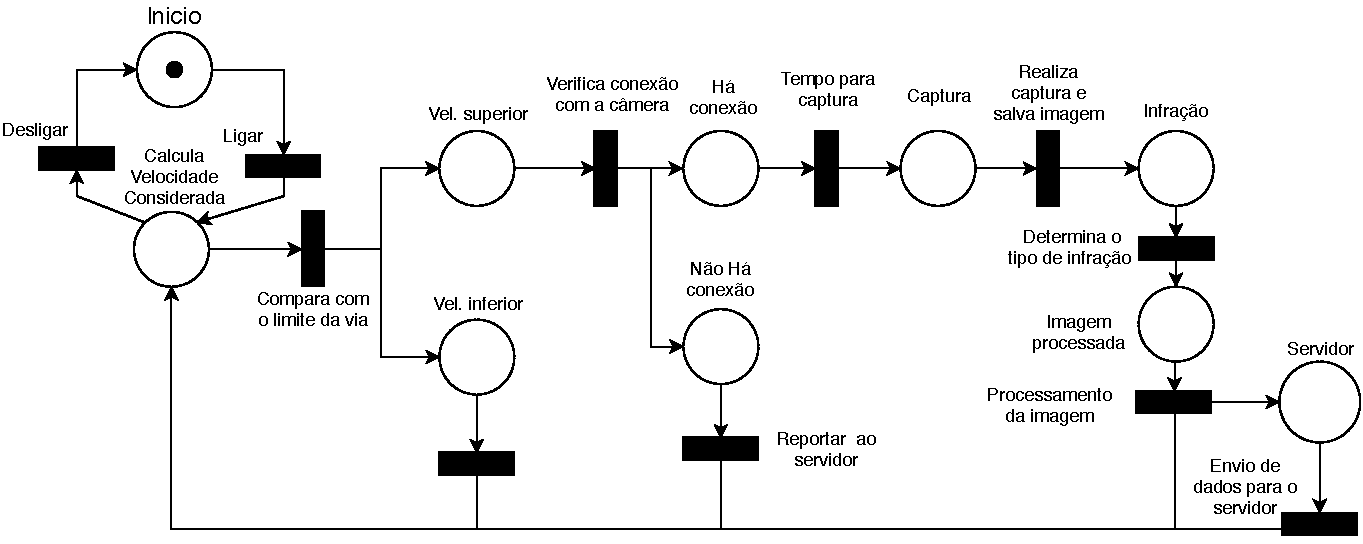
\includegraphics[scale = 0.54]{figuras/PetriNet_Infracao-3.pdf}
    \caption{Rede de Petri que representa a \emph{thread} executada no código de controle referente à infração e captura.}
    \label{Petricaptura}
    \end{figure}. 

Conforme a {Figura \ref{Petricaptura}}, inicialmente encontramos a velocidade considerada e comparamos com a velocidade regulamentada pela via. Se ocorre a infração, é utilizada a velocidade medida e a distância do local de detecção até a área de captura para dar tempo do veículo chegar em uma boa posição para a captura da imagem. Para a câmera ser acessada, utiliza-se um função do \emph{OpenCV} com protocolo de comunicação, usuário, senha e o IP em que ela se encontra. Com isso a captura é feita e salva em uma pasta onde se encontra o banco de imagens de cada dia na \emph{Raspberry Pi}. Por fim a imagem é enviada para a função de pré-processamento de imagens, visto na Seção \ref{procimag}, e posteriormente enviada ao servidor, visto na Seção \ref{serv}.

\subsection{Envio de dados para o servidor} \label{serv}
    
O servidor recebe alguns dados do veículo que estiverem transitando acima do limite estabelecido na via. Foi definido que os dados enviados são: 

    \begin{itemize}
        \item ID do radar: Identificação do equipamento utilizado, mediante numeração estabelecida pela entidade de trânsito. Este dado é do tipo inteiro;
        \item Velocidade regulamentada: Velocidade limite para  local da via determinada pelas normas do CONTRAN\cite{conatran}. Este dado é do tipo inteiro;
        \item Velocidade medida: Velocidade  do veículo calculada pelo equipamento. Este dado é do tipo inteiro;
        \item Velocidade considerada: Velocidade medida subtraída pelo erro máximo admitido previsto na legislação metrológica. Este dado é do tipo inteiro;
        \item Infração: Natureza da infração cometida. Estes dados são do tipo inteiro enviados por enumeração, onde 0, 1 e 2 correspondem respectivamente a média, grave e gravíssima;
        \item Imagens: As imagens tanto em escala de cinza do carro quanto a imagem pré processada para reconhecimento da placa são enviadas no formato base64, método para codificação de dados para transferência na Internet;
        \item Câmera: Retorna se a câmera está ou não funcionando corretamente. Este dado será do tipo \emph{boolean}, sendo \emph{True} para correto funcionamento e \emph{False} para mau funcionamento. 
        \item \emph{Raspberry}: Retorna se o NRF24L01 está ou não funcionando corretamente. Este dado será do tipo \emph{boolean}, sendo \emph{True} para correto funcionamento e \emph{False} para mau funcionamento.
        \item USRP: Retorna se o USRP está ou não funcionando corretamente.  Este dado será do tipo \emph{boolean}, sendo \emph{True} para correto funcionamento e \emph{False} para mau funcionamento.
        \item Funcionamento do radar: Retorna se o radar em geral está funcionando corretamente. Este dado será do tipo \emph{boolean}, sendo \emph{True} se todos estão funcionando e \emph{False} se um ou mais componentes não estão funcionando.
        \end{itemize} 
        
 O protocolo que faz comunicação entre a \emph{Raspberry Pi 3} e o servidor é o \emph{Advanced Message Queuing Protocol} (AMQP). No código, o envio de dados para o servidor foi dividido em dois, sendo o primeiro uma \emph{thread} chamada apenas dentro da função de processamento de imagens, para envio de dados referentes à multa, e a outra \emph{thread} executa e confere a operacionalidade dos componentes. A decisão de enviar o pacote de dados referentes à infração através de uma \emph{thread} é pelo fato do tamanho das imagens provocar uma demora em torno de 8 segundos, e com isto executando paralelamente, não interfere no restante do código de controle. Já a \emph{thread} de operacionalidade sempre está rodando e informando sobre a operacionalidade dos componentes, para o caso de algum defeito o responsável já saber onde está o problema. \par
 Em relação às imagens, as duas enviadas no \emph{payload} de infração sofrem uma redução para 300 kB através de uma função de compressão e otimização de imagem que não interfere no reconhecimento da placa, fazendo com que o pacote seja menor e o tempo de envio também. Posteriormente são convertidas em base 64 e enviada para o \emph{localhost} onde se encontra a fila do maestro.

\subsection{\emph{Cooler}} 
O \emph{cooler} dimensionado deve ficar ligado durante o dia e desligado durante a noite. Para fazer seu controle, foi criada uma \emph{thread} em paralelo com as demais onde foi utilizado o segundo canal do relé, que determinado em código, é ativado entre as 7 horas da manhã até as 18 horas. O módulo relé de 2 canais ativa em modo baixo, por isso para ligar o \emph{cooler}, deve-se setar o pino em \emph{low}.

\section{Processamento de imagem} \label{procimag}

Este processo tem como objetivo tratar a imagem capturada pela câmera de modo que possa ser reconhecido a placa do veículo, facilitando no reconhecimento dos caracteres que é feito pelo servidor. Ao final deste processo são geradas duas imagens, uma contendo apenas a transformação de escala em cinza e a outra imagem é da placa a ser processada. O procedimento para a localização de placas de carro é mostrado na Figura \ref{fig:proc_img}.
%%diagrama do processo
\begin{figure}[H]
    \centering
    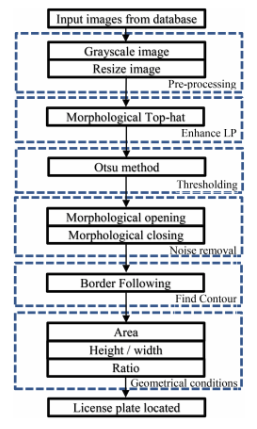
\includegraphics[scale = 0.6]{figuras/procimagpng.png}    \caption{Procedimentos e operações morfológicas para localização de placas de carro em imagens \cite{yepez2018improved}.}
    \label{fig:proc_img}
\end{figure}
A Figura \ref{fig:proc_img} trata da sequência de operações relacionadas a localização da placa de carro em uma imagem. 

\begin{figure}[H]
    \centering
    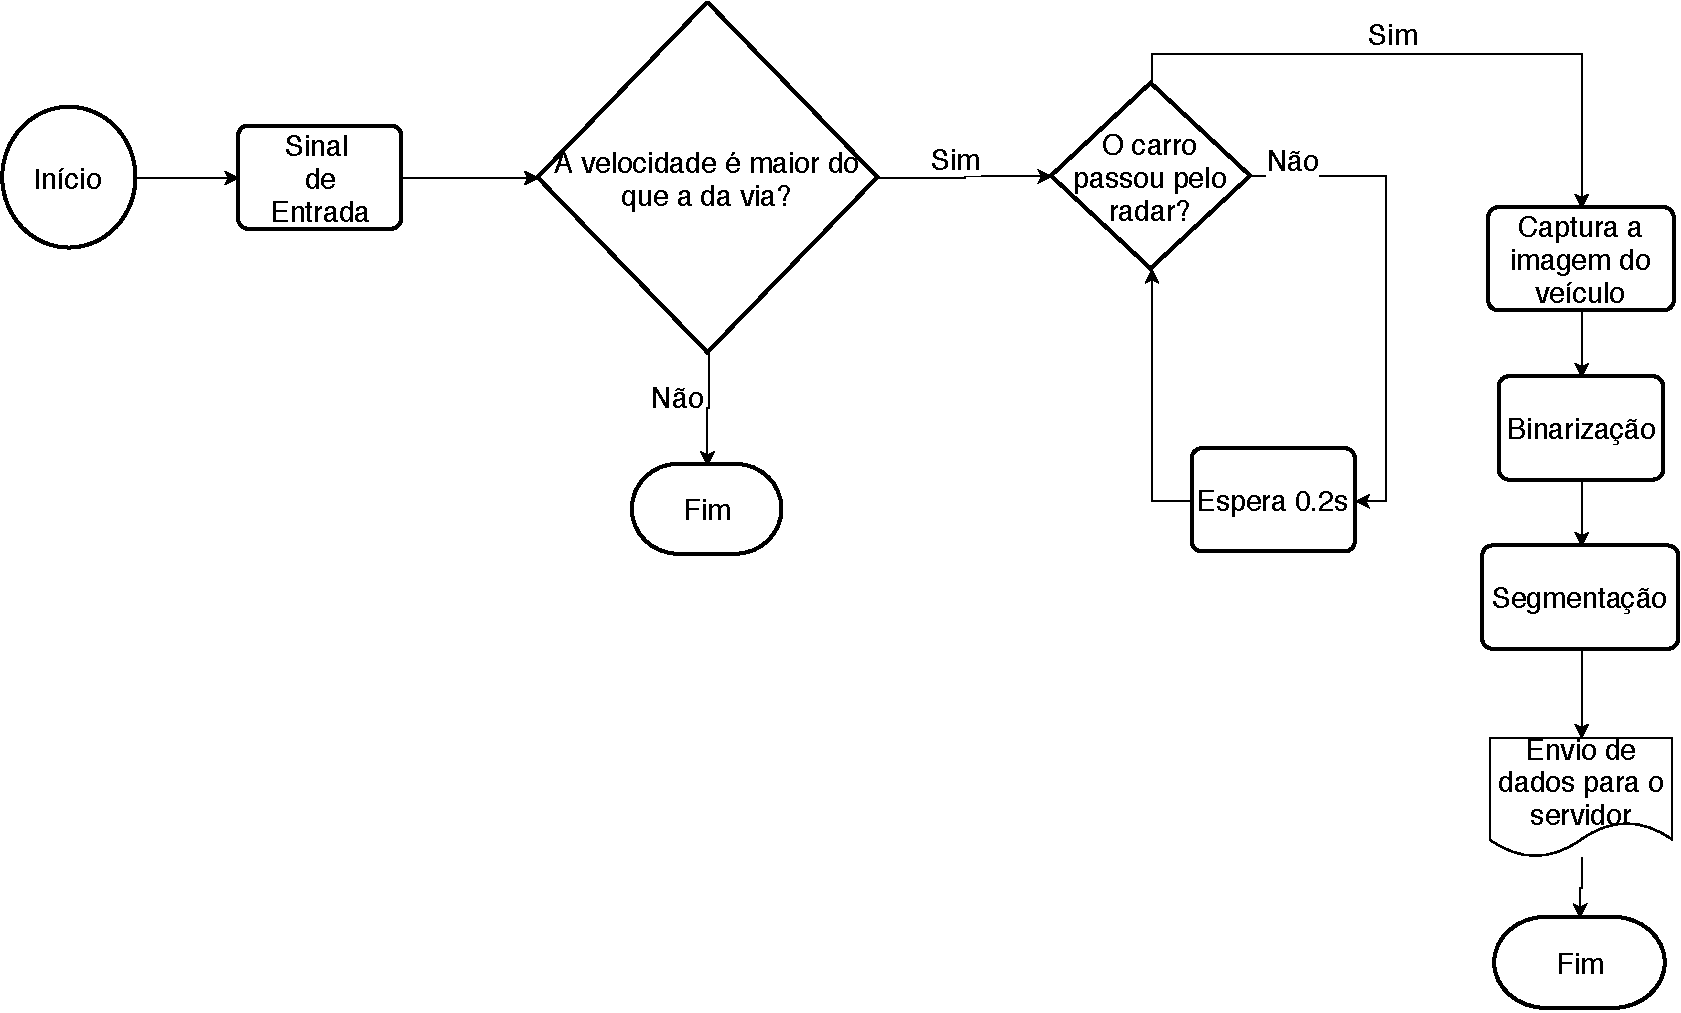
\includegraphics[scale=0.4]{figuras/Diagrama_logico_imagem.pdf}
    \caption{Etapas do processamento de imagem a serem realizadas e seus elementos responsáveis pela execução. A câmera faz a aquisição da imagem, a \emph{Raspberry Pi 3} faz o pré-processamento, segmentação e representação, e o servidor realiza o reconhecimento da placa \cite{yepez2018improved}.} 
    \label{processamento_imagem}
\end{figure}

\begin{itemize}
    \item \emph{Grayscale image}: Consiste em transformar a imagem em escala de cinza;
    \item \emph{Top Hat}: Extração de elementos e detalhes da imagem, consistindo na subtração da imagem obtida na primeira etapa após uma operação de abertura com elemento estruturante no formato de um retângulo;
    \item Otsu \emph{method}: Processo de binarização através da técnica de Otsu que visa calcular o histograma de uma imagem e tomar como limiar. Para um processo de binarização, a metade do índice de dois picos para então usar este valor como limite; 
    \item \emph{Morphological opening/closing}: Remoção de ruído, através da sequência de abertura e fechamento para que objetos que não tem correspondência com o formato da placa sejam filtrados; 
    \item \emph{Border following}: Imagem foi varrida em busca de objetos que tem estrutura semelhante ao padrão utilizado nas outras etapas, destacando-os em seguida através de um algoritmo detector de borda, mais precisamente, o algoritmo \emph{Canny edge}. 
\end{itemize}
    
Todas as etapas foram implementadas através da plataforma OpenCV na linguagem de programação \textit{Python} \cite{yepez2018improved}\cite{gonzalez2007digital}.


\subsection{Transformação para escala de cinza}

A escala de cinza é a transformação de uma imagem colorida, em que cada pixel é transformado em um valor que corresponde a uma escala do branco ao preto, diminuindo a quantidade de informação na imagem que não é útil para as sequências das operações. Esta transformação foi feita diretamente pelas configurações da câmera, não sendo necessário nenhum comando no código para o processamento do mesmo. 

Uma imagem com três canais de cores forma, RGB, por exemplo, endereça cada pixel através de duas dimensões sendo que cada elemento contém três valores, formando, assim, uma matriz com tamanho $M\,x\,N\,x\,P$ sendo P um vetor de três posições. Para um imagem com resolução de 1920 por 1080 \emph{pixels} têm-se uma matriz com $1920\,x\,1080\,x\,3$ o que implica, em um objeto, de tamanho 6220800 enquanto que uma imagem em escala de cinza condiz com um objeto com tamanho 2073600. Outro ponto condicionado a utilização de imagens em escala de cinza é o efeito de operações morfológicas de acordo com \cite{yepez2018improved}. As Figuras \ref{cinza} e \ref{original} mostram a transformação para escala de cinza de uma imagem colorida capturada pela câmera. 

\begin{figure}[H]
    \centering
     \begin{subfigure}{0.8\textwidth}
        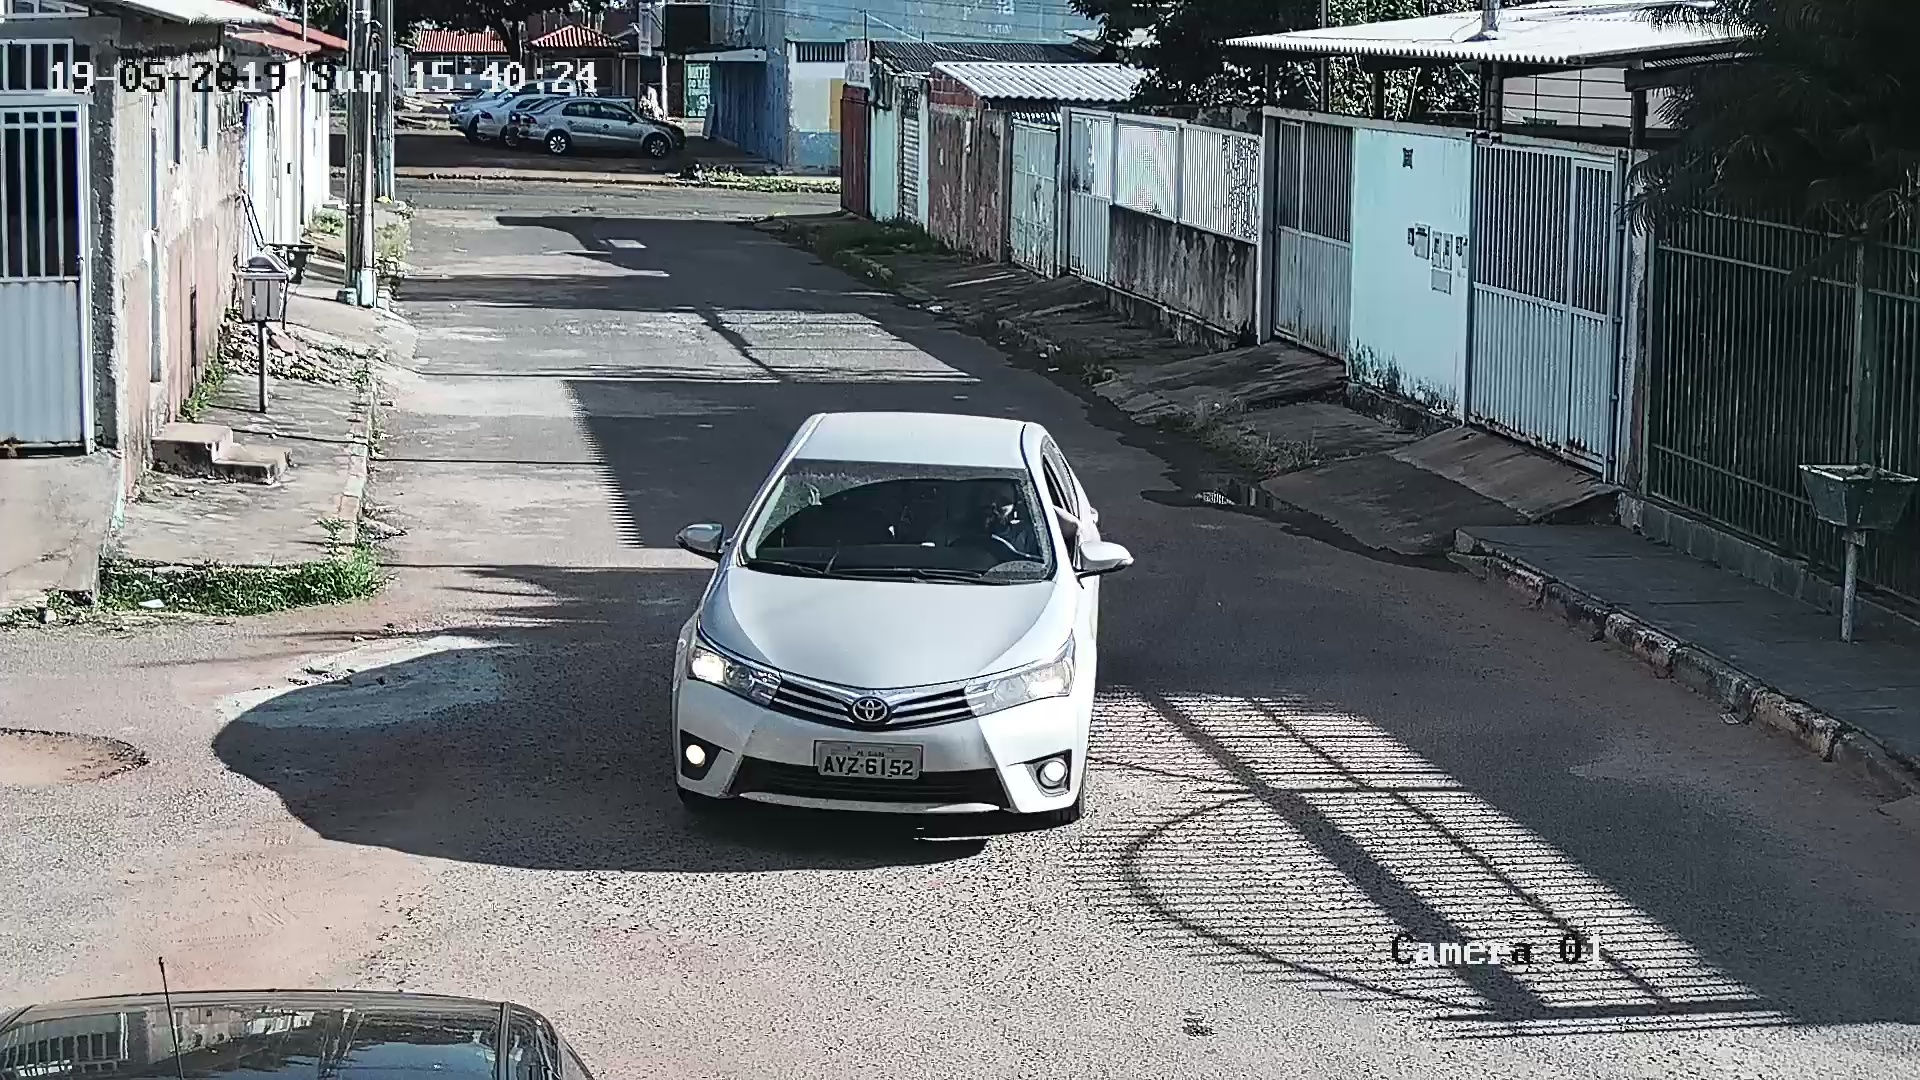
\includegraphics[width=\textwidth]{figuras/transforma2.jpg}
        \caption{Imagem original}
          \label{original}
      \end{subfigure}
        \hfill
      \begin{subfigure}{0.8\textwidth}
        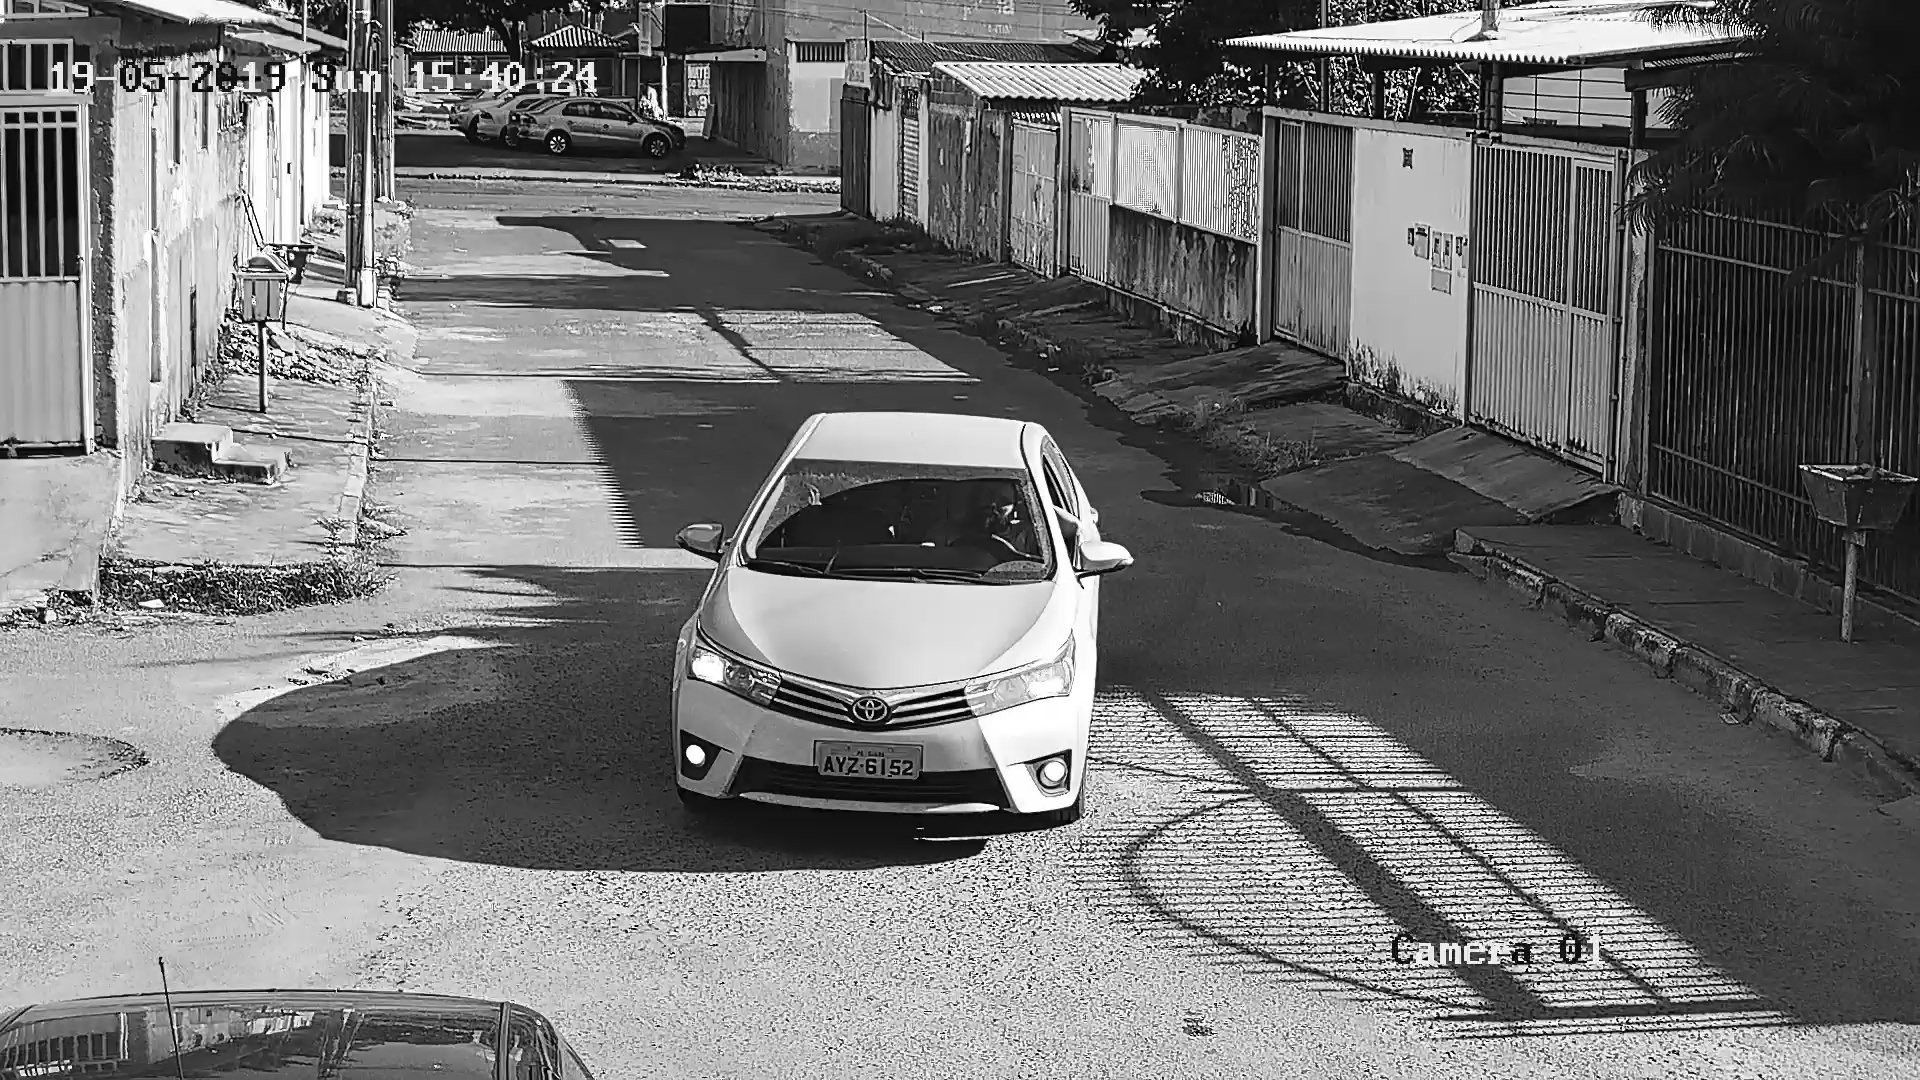
\includegraphics[width=\textwidth]{figuras/transforma2_1.jpg}
        \caption{Imagem original transformada em escala de cinza}
          \label{cinza}
      \end{subfigure}
        \hfill
       
\end{figure} 


\subsubsection{Binarização}
A partir de um aplicação de um limiar na imagem com escala em cinza, os \emph{pixels} com valores maiores que este limiar recebem o valor máximo da escala de cinza e os \emph{pixels} com valor menor que o limiar, recebem o valor mínimo  \cite{gonzalez2007digital}.

\subsection{Resultados após processamento de imagem}


Na figura \ref{fig1:demarcada} foram demarcados vários elementos para tentar reduzir a quantidade de objetos, aplicando um filtro de borramento na imagem original para diminuir a quantidade de transições entre objetos candidatos a placa de carro e o fundo da imagem. A próxima etapa a ser feita é classificar o objeto na imagem em placa e não placa de carro, para, em seguida realizar o reconhecimento de caracteres.

Como elemento estruturante para as operações morfológicas foi utilizado um retângulo calculado de acordo com as especificações da câmera, sendo imagem com resolução de 1290 por 720 \emph{pixels} a uma distância aproximada de 10 m . Com ângulo de abertura horizontal e vertical de 34º e 19º, respectivamente, ocasiona em um plano com dimensionamentos de acordo com as Eqs. \ref{dimensoes1}:
\begin{equation}
    2\,d\,cos(\theta_{h} /2) = 19,12 m, 
    2\,d\,cos(\theta_{v} /2) = 19,72 m.
    \label{dimensoes1}
\end{equation}

As Eq. \ref{dimensoes1} permitem mensurar a densidade linear de \emph{pixels} por metro, sendo, 66,93 pixels/m para a horizontal e 36,5 pixels/m para a vertical.

Sabendo-se que a dimensão da placa do carro é de 0,4 m por 0,15 m estimou-se o tamanho do elemento estruturante multiplicando-se a densidade de \emph{pixels} obtida com o tamanho da placa obtendo-se uma matriz de tamanho 27 por 5, esse tamanho foi utilizado para formar um elemento estruturante de formato de um retângulo para ser utilizado na aplicação da operação morfológica \emph{Top Hat}, como mostra a Figura \ref{fig:three graphs}.

\begin{figure}[H]
     \centering
     
     \begin{subfigure}{0.7\textwidth}
         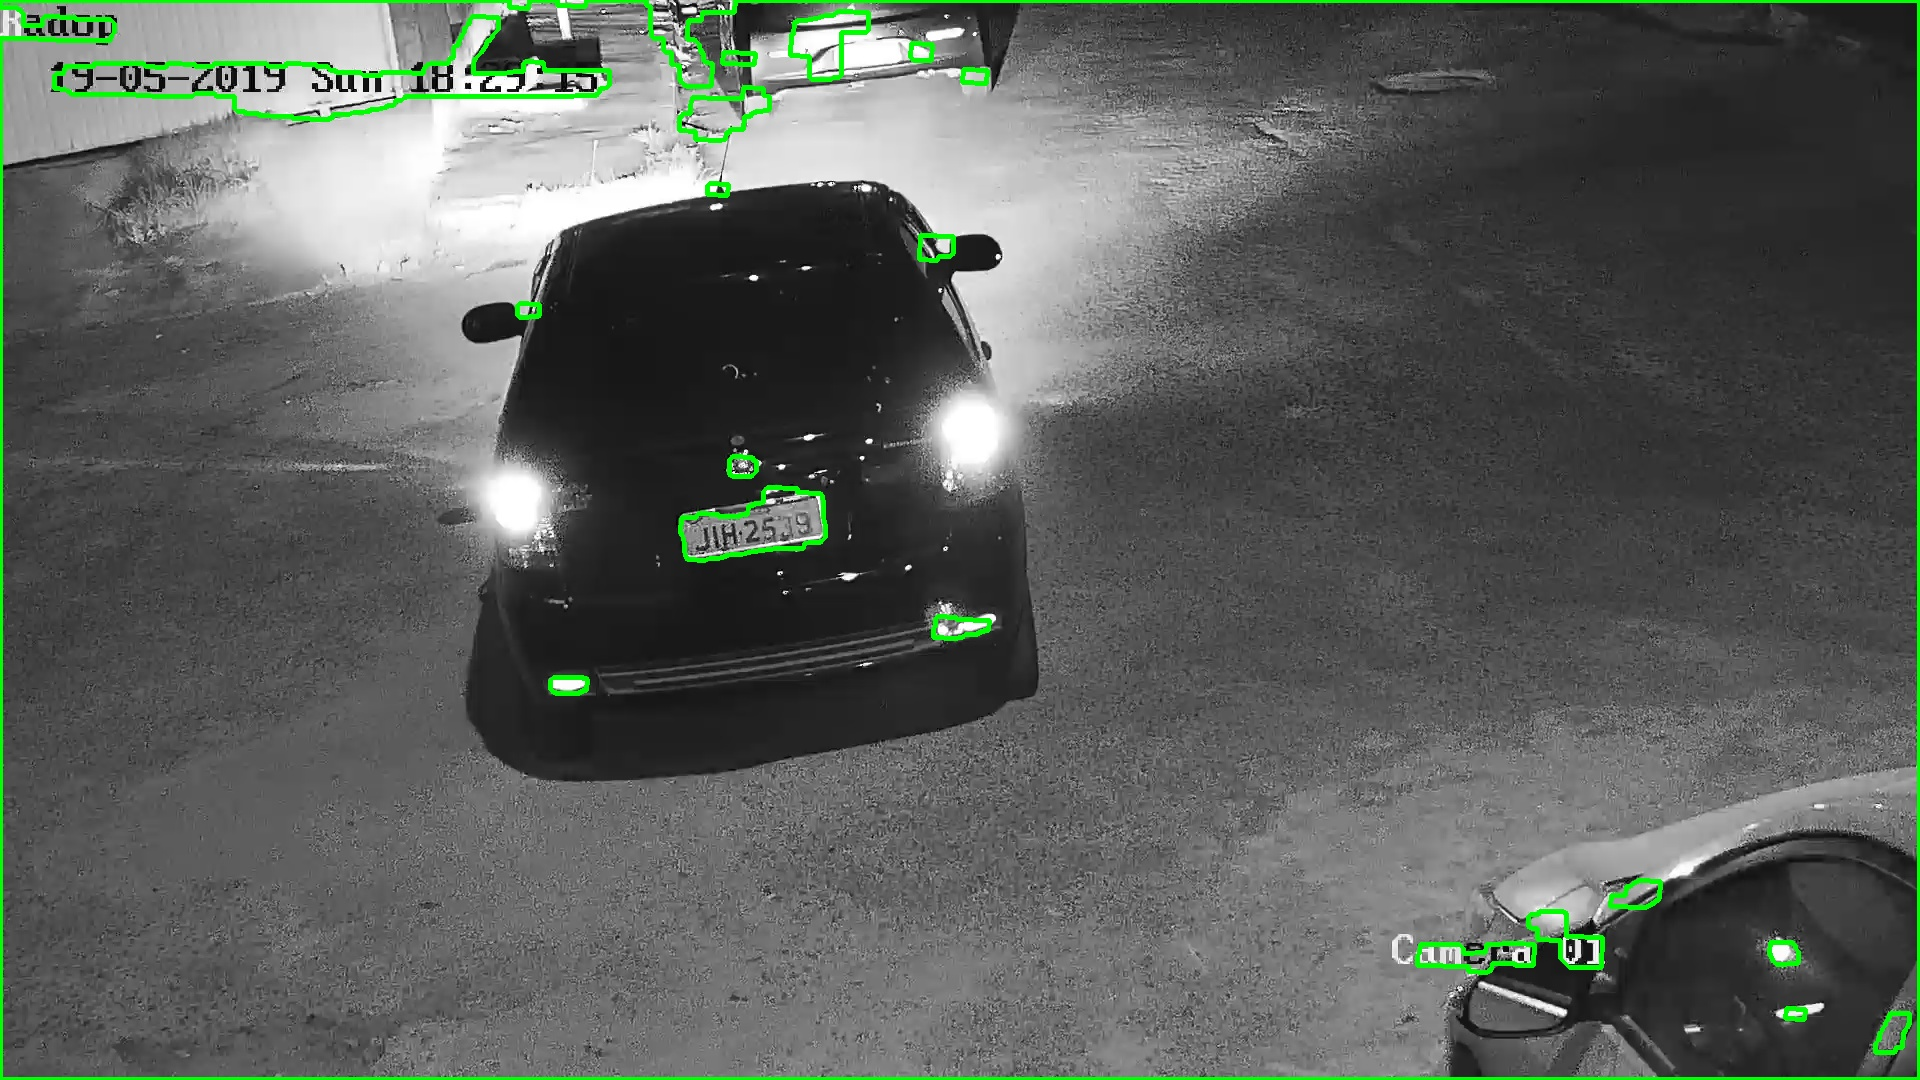
\includegraphics[width=\textwidth]{figuras/img_origin_n.jpg}
         \caption{}
         \label{fig1:demarcada}
     \end{subfigure}

     \begin{subfigure}{0.7\textwidth}
         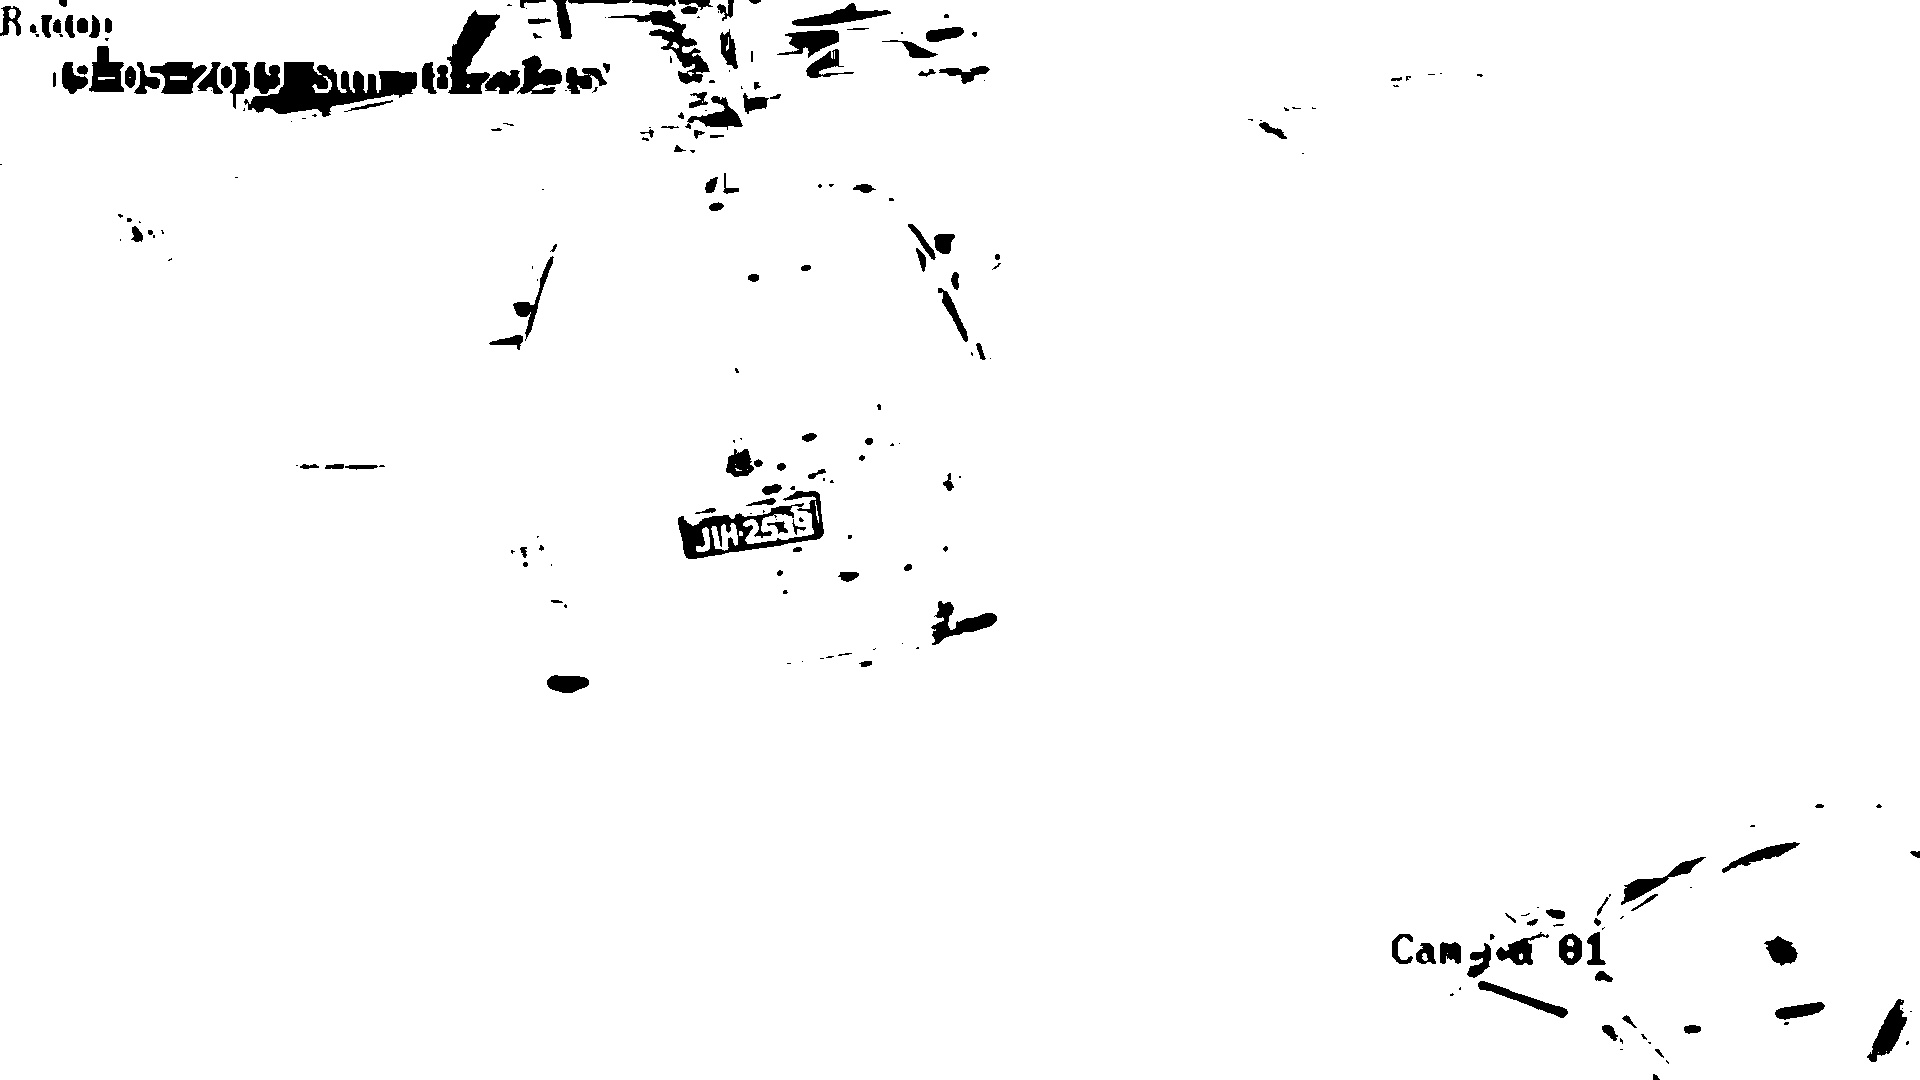
\includegraphics[width=\textwidth]{figuras/thr_n.jpg}
          \caption{}
         \label{fig2:thresh}
     \end{subfigure}

  
\end{figure}

\begin{figure}[H] \ContinuedFloat
    \centering
    \begin{subfigure}{0.7\textwidth}
         
\includegraphics[width=\textwidth]{figuras/op_cl_n.jpg}
          \caption{}
         \label{fig3:op_cl}
         
     \end{subfigure}
     \caption{\ref{fig1:demarcada} mostra marcação de locais possíveis onde pode haver uma placa de carro, \ref{fig2:thresh} corresponde a \emph{Top hat} mais binarização de Otsu e \ref{fig3:op_cl} mostra operações de abertura e fechamento.}
    \label{fig:three graphs}
\end{figure}
